\chapter{Applications to named entity recognition and word sense disambiguation} 
\label{chap:wsd}
\begin{abstractchap}
This chapter presents the experiments we performed as applications of the proposed model. On the first subsection, we use well-known methods to solve named entity recognition while using fusion enriched representation spaces. We show that these kinds of representations, leveraging heterogeneous information and alleviating its data sparsity, are useful to improve the performance of the task. Indeed, our results on three different datasets using enriched representations are better than those of the baselines we propose, and more importantly, our results show that the combination of textual features indeed improves the performance compared to single feature and the trivial feature concatenation. We also give a detailed analysis into how the fusion operations get to improve the performance of the task at hand.

In the second subsection, we change the NLP task to word sense induction and disambiguation. First, we apply the same fusion operations as before to solve the task using an existing literature approach. Our experiments on two different corpora show that the improvements shown in named entity recognition are consistent in word sense induction and disambiguation. Secondly, we propose a method to exploit the structure of the network within our linguistic model. 
Although this approach has been studied before, we improve over the previous  literature results while having a reduced number of parameters and employing heterogeneous features to solve the task. We also analyze the results obtained according to the  type of word studied, whether nouns or verbs, and according to the effect of the use of either lexical or syntactical information.


%Secondly, in the second section of the chapter, we explore the use of well-known multi-modal fusion techniques to solve two prominent Natural Language Processing tasks. Specifically, we focus on solving Named Entity Recognition and Word  Induction and Disambiguation by applying feature-combination methods that have already shown their efficiency in the multi-media analysis domain. We present a series of experiments employing fusion techniques in order to combine textual linguistic features. 
%Furthermore, we perform an extensive analysis on the importance of each feature relevance with respect to the senses and classes discovered in WSI/WSD and NER, respectively.

\end{abstractchap}

\minitoc
\section{Introduction}
In this applications chapter we set to solve two natural language processing tasks using as data source corpora in the form of the model described in Chapter \ref{chap:ling_net}. We address the tasks of Named Entity Recognition (NER) and Word Sense Induction and Disambiguation (WSI/WSD). Both tasks are located on the  semantics sub-domain of NLP. 

These experiments represent the third and final contribution of this thesis, after introducing the theoretical fusion enriched model in the previous chapter. Indeed, this contribution is the continuation of our set of propositions, as shown in Figure \ref{fig:main_diag2}. We employ both a fusion enriched and a raw hypergraph network based on benchmark corpora to validate the utility of our proposals.

The general objectives of the experiments described below are two: (1) to test the effectiveness of using fusion enriched representations to solve NLP tasks, while combining heterogeneous information and densifying the feature space;  and (2), to leverage the structure of a network built using the hypergraph structure described before.

 %By making use of the network we want to test the effectiveness of using different types of linguistic features. 
There are two main parts  in this chapter. First we address NER, we study how the different types of fusion operations affect the performance of the task. We train well-known classification algorithms with representations obtained from fusion operations.  According to our results, we find that it is indeed interesting to combine different types of features into a single representation space. We also delve into a result's analysis to try to understand the reason behind the improvement using fusion techniques.

The second part deals with WSI/WSD. This subsection is divided in two segments. First, once we determined that combining features is interesting for NER, we want to verify that this combined representations are indeed useful for other NLP tasks, such as WSI/WSD. As before, we use a literature learning technique with the representation obtained by the combination of available features. Our results show that the fusion enrichment is useful also to solve WSI/WSD.

Secondly, we leverage the structure within the hypergraph resource to solve WSI/WSD. Briefly, the goal is to detect important words, according to their connections with other words, and extract their neighborhood to determine possible senses  within the network. While this method has been used before, we improve the performance and reduce the number of parameters employed by those literature methods. We also study the effect of using different types of linguistic information, namely lexical and syntactic contexts.

At the end of the chapter we conclude by discussing the experiments performed, their limitations and  future improvements and further research. 

\begin{figure}
\centering
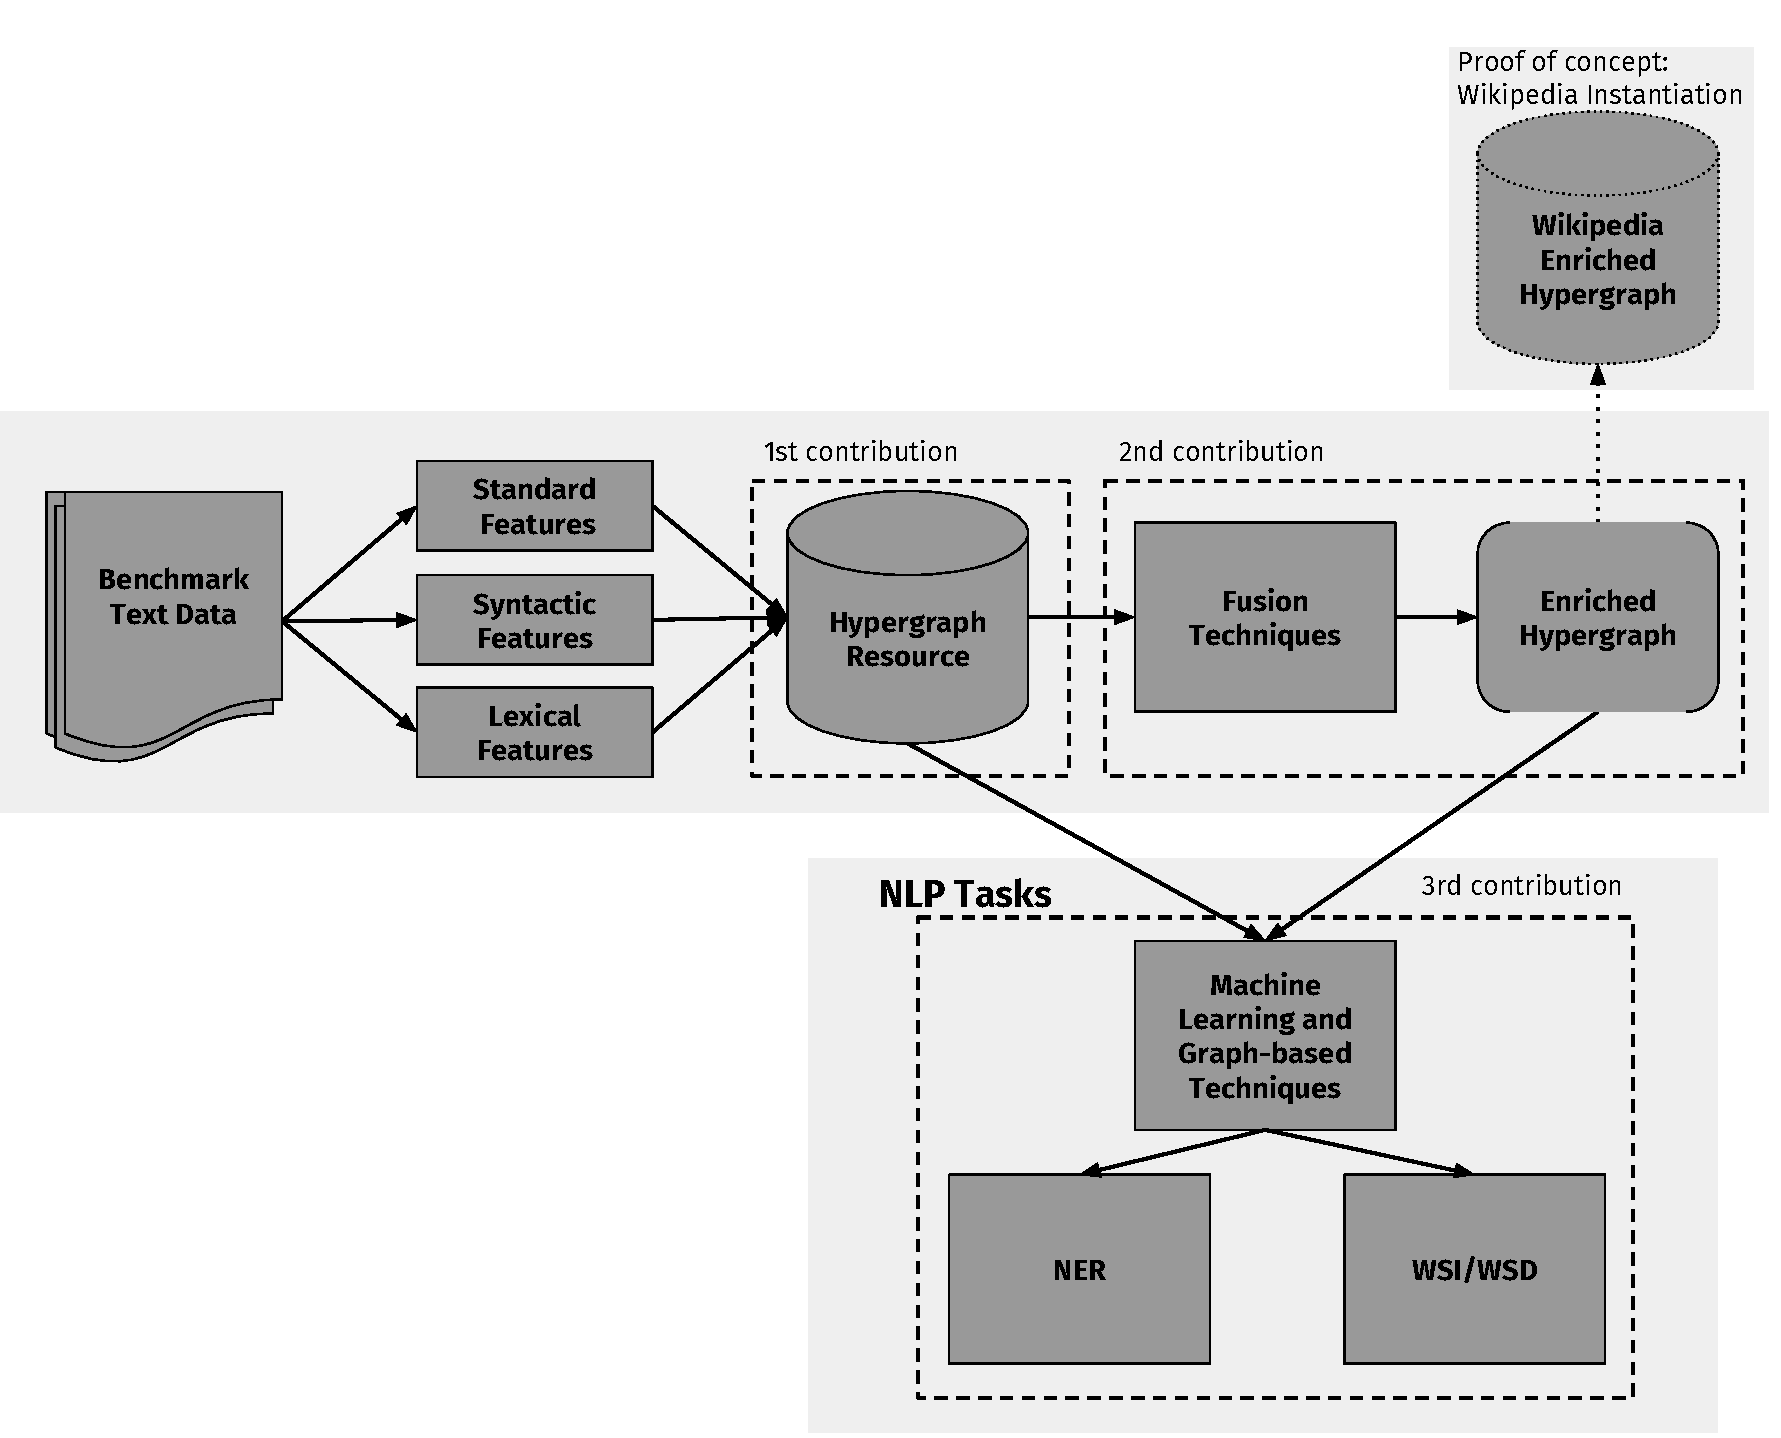
\includegraphics[width=.7\linewidth]{images/Chapitre4/main_diag2.pdf}
\caption{Complete description of the three contributions of this work. In this chapter we focus on  WSD/WSI and NER as applications of the model proposed.}
\label{fig:main_diag2}
\end{figure}

\section{First Application: Named Entity Recognition}
\label{sec:ner}


 NER goal is to automatically discover, within a text, mentions that belong to a well-defined semantic category. The classic task of NER involves detecting, within a text, entities of type Location (LOC), Organization (ORG), Person (PER), Miscellaneous (MISC), or if the term is not an even an entity, assigning them a (O) label. The task is of great importance for more complex NLP systems, e.g, relation extraction, opinion mining \cite{nadeau2007survey}.  
 
 Generally, two common solutions to NER involve the use of matching patterns, created manually or extracted in a semi-automatically fashion\cite{gupta2015distantly}; or more popularly, by training a supervised machine learning algorithm with large quantities of annotated text \cite{mining12Book} . The latter being the currently more popular solution to this task. As is usual with other NLP tasks, NER  requires textual features to represent words in order to determine their role within a phrase. We propose to build representations based on our fusion enriched hypergraph model.


Usually, representations employed for NER are obtained from the surrounding context of the words in the  input corpus. Mainly,  two types of representations are used: lexical and syntactic. As we know, the first type requires no extra information than that contained already in the analyzed text itself. The second type, syntactic features  are based on part of speech tags, phrase constituents information, and syntactical functionality between words, the later portrayed by syntactical dependencies. Likewise, there are specific features that are particular to one task are also be employed.


The main intuition of these experiments is that word similarities may be found at different levels according to the type of features employed. In order to exploit these similarities, we leverage our fusion enriched framework. Specifically, in our experiments, we try to mutually complement independent representations by utilizing said fusion techniques to generate a single feature space that improves the performance of NER, specially compared to the using features independently and the trivial feature concatenation (early fusion). Consequently, the main goal is to assess the effectiveness of simple, yet untested fusion techniques and their combination.

%The rest of the chapter is organized as follows: in section \ref{chap6:back}, we go into further details about fusion techniques. 
%%as well as its application in the NLP domain. 
%We introduce the fusion operators that we use in our experiments in section \ref{chap6:application}. Then, in section \ref{chap6:expes} we show the effectiveness of the presented methods by testing them on NER and WSI/WSD and their respective datasets. Finally, in section \ref{chap6:conclusion} we present our conclusions and future directions to explore. A more general overview on fusion for multimedia analysis can be found in \cite{AtreyHEK10}.


We consider the first three types of fusion techniques described in subsection \ref{sec:fusion} (early fusion, late fusion and cross fusion) as the building blocks to the experiments we conduct.  While we work with a single modality, i.e., textual data, we consider the different kinds of features extracted from it as distinct modalities. Our intuition being that the semantic similarities among words in these different spaces can be combined in order to exploit the latent complementarity between the lexical and syntactical representations. We also find new combinations empirically. Nonetheless, as we will show, their effectiveness replicates to different datasets and NLP tasks. 

The specific methods used to solve both NER and WSI/WSD (in the following subsection) are already known to be robust. Our work focus specially on the generation of new representation spaces.
% Using well-proven methods to solve both WSI/WSD and NER, so that the learning part of our experiments is known to be robust.
%The fusion should therefore improve the performance of the NLP tasks at hand, first NER and later on WSI/WSD

\subsection{Fusion Enriched Representations}
\label{chap6:application}
 Our first goal in this subsection is to assess the effectiveness of the classic fusion methods and then, as a second goal, to propose new combinations that yield better outcomes in terms of performance than the simpler approaches. The new combinations are found through experimentation. Nonetheless, as we will show, their effectiveness replicates to different datasets and NLP tasks. 





\begin{figure}[t]
\centering
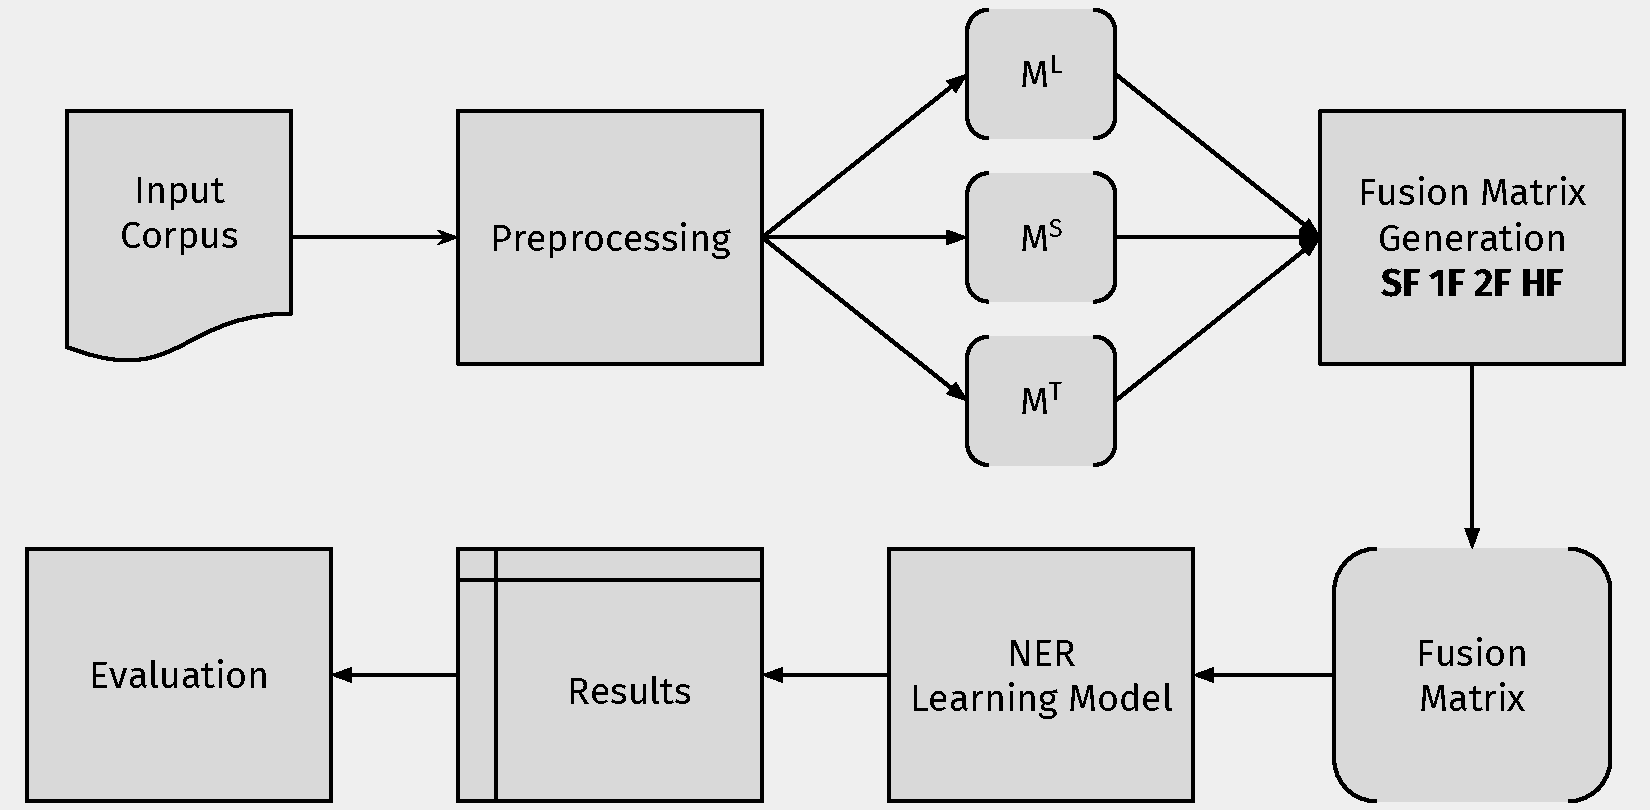
\includegraphics[width=0.85\linewidth]{images/Chapitre4/diag_metodoNER.pdf}
\caption{Steps followed on our fusion-enriched representations for NER  experiments. First the corpus is preprocessed, then features are extracted from the text. A fusion matrix is generated, which in turn is used as input to a learning algorithm. Finally, the system yields its results and to be analyzed.}
\label{fig:diagmetodo}
\end{figure}

The experiments we carry on consist in generating fusion matrices that will serve as input to a learning algorithm in order to solve NER. These input feature matrices are based upon lexical, syntactical, or other NER standard types of representation. The procedure can be sen in Figure \ref{fig:diagmetodo}.

\paragraph{Representation Spaces}\label{sec:rep_spaces}
In  Chapter \ref{chap:ling_net} we presented the fusion operators to be used in our experiments. Below we detail the three types of features matrices used to generate the fusion-enriched combinations that describe the words of the corpus tested.
\subparagraph{Lexical Matrix (L)}
For each token in the corpus, we use a lexical window of two words to the left and two words to the right, plus the token itself. Specifically, for a target word $w$, its lexical context is $(w_{-2}, w_{-1}, w, w_{+1}, w_{+2})$. This type of context features is typical for general systems studying the surroundings of a word and in particular for the named entity recognition task \cite{Daume2006,Nothman2009,RatinovR09}. 
 We retake the example phrase from \cite{LevyG14}, the lexical-based features of the phrase \textit{Australian scientist discovers start with telescope}, are shown in Table \ref{tab:lex-contextos}.
 
\begin{table}[ht]
\centering
\begin{tabular}{ll}
\hline 
 \textbf{Word} & \textbf{Features} \\ 
\hline 
Australian & word:Australian, word+1:scientist, word+2:discovers\\ 
scientist  &  word-1:Australian, word:scientist, word+1:discovers, word+2:star\\ 
discovers & word-2:Australian, word-1:scientist, $\dots$, word+2:telescope \\ 
star & word-2:scientist, word-1:discovers, word:star, $\dots$, word+2:telescope \\ 
with & word-2:discovers, word-1:star, word:with, word+1:telescope \\ 
telescope  &  word-2:star, word-1:with, word:telescope \\ 
\hline \
\end{tabular} 

\caption{Lexical features corresponding to the phrase \textit{Australian scientist discovers start with telescope}.}
\label{tab:lex-contextos}
\end{table} 

\subparagraph{Syntactical Matrix (S)}
Based on the syntactic features used in   \cite{LevyG14,Panchenko2017}, we derive contexts based on the syntactic relations a word participates in, as well as including the part of speech (PoS) of the arguments of these relations. Formally, for a word $w$ with modifiers $m_1, \dots, m_k$ and their corresponding PoS tags $p_{m_1}, \dots, p_{m_k}$; a head $h$ and its corresponding PoS tag $p_h$, we consider the context features $(m_1, p_{m_1}, lbl_1), \dots, \allowbreak (m_k, p_{m_k}, lbl_k), \allowbreak (h,p_h,lbl\_inv_h)$. In this case, $lbl$ and $lbl_{inv}$ indicate the label of the dependency relation and its inverse, correspondingly. Using syntactic dependencies as features should yield more specific similarities, closer to synonymy, instead of the broader topical similarity found through lexical contexts.

For the phrase \textit{Australian scientist discovers start with telescope} the dependency-based context is shown in Table \ref{tab:syn-contexts}.
\subparagraph{NER Standard Features Matrix (T)}
The features used for NER are based roughly on the same as those used in \cite{Daume2006,Balasuriya2009}. The feature set consists of: the word itself, whether the word begins with capital letter, prefix and suffix up to three characters (also within a window of two words to the left and two words to the right), and the PoS tag of the current word. These features are considered to be standard in the literature. We note that the matrix generated with these features is exclusively used in the experiments regarding NER.	

\begin{table*}
\centering
\begin{tabular}{ll}
\hline 
 Word & Contexts \\ 
\hline 
Australian & scientist/NN/amod\_inv \\ 
scientist  &  Australian/JJ/amod, discovers/VBZ/nsubj\_inv\\ 
discovers & scientist/NN/nsubj, star/NN/dobj, telescope/NN/nmod:with \\ 
star & discovers/VBZ/dobj\_inv \\ 
telescope  &  discovers/VBZ/nmod:with\_inv \\ 
\hline \
\end{tabular} 
\caption{Syntactic contexts corresponding to the phrase \textit{Australian scientist discovers start with telescope}.}
\label{tab:syn-contexts}
\end{table*}


\paragraph{Learning Methods}
NER being a supervised learning task, we use an averaged structured perceptron  \cite{Collins2002,Daume2006} (see Section \ref{sec:perceptron}) to determine the tags of the named entities. We considered logistic regression and linear SVM. For the main experiments, we chose the perceptron because of its performance and the lower training time. On the other hand, for the analysis of the results, we use a logistic regression as it is considerably easier to interpret its results, keeping in mind that our goal is to give some insights regarding the usefulness of our fusion methods.




\subsection{Experiments and Evaluation}
\label{chap6:expes}

We experiment with the four levels of fusion discussed before: Single Features (SF), First-degree Fusion (1F), Second-degree Fusion (2F) and Higher-degree Fusion (HF). The representation matrices for NER come from lexical context features $\mlex$, syntactical context features $\msyn$ or standard features $\mstd$.  On the other hand, experiments on WSI/WSD exclusively employ matrices $\mlex$ and $\msyn$.

We recall that our first goal is to compare the efficiency of the primary  fusion techniques applied to   named entity recognition. Then, we empirically determine a fusion combination operator able to leverage the complementarity of the features used.

To this end, we evaluate the aforementioned 4 fusion levels. We note that the fusion combinations in the third and fourth level (2F and HF) are proposed based on the results obtained in the previous levels. In other words, in order to reduce the number of experiments, we restrict our tests to the best performing configurations. This is due to the large number of possible fusion combinations that can be tested.
% (an argument to a fusion operation may be any valid output of a second fusion operation).



\paragraph{Preprocessing}

As is usual when preprocessing text before performing named entity recognition, \cite{RatinovR09}, we normalize tokens that include numbers. For example, the token 1980 becomes *DDDD* and 212-325-4751 becomes *DDD*-*DDD*-*DDDD*. This allows a degree of abstraction to tokens that contain years, phone numbers, etc. We do not normalize punctuation marks.

\paragraph{Features}
The linguistic information we use is again extracted with the Stanford's CoreNLP parser. We recall that the features used for these experiments on NER are those described before: lexical, syntactic and standard features, i.e., $\mlex$, $\msyn$, and $\mstd$, respectively. 

\paragraph{Test Datasets}We work with three corpus coming from different domains:
\begin{itemize}
\item [(1)] CoNLL-2003 (CONLL): This dataset was used in the language-independent named entity recognition CoNLL-2003 shared task \cite{SangM03}. It contains selected news-wire articles from the Reuters Corpus. Each article is annotated manually. It is divided in three parts:  training (\textit{train}) and two testing sets (\textit{testa} and \textit{testb}). The training part contains 219,554 lines, while the test sets contain 55,044 and 50,350 lines, respectively. The task was evaluated on the \textit{testb} file, as in the original task.
\item [(2)]WikiNER (WNER): A more recent dataset \cite{Nothman2009} of selected English \allowbreak Wikipedia articles, all of them annotated automatically with the author's semi-supervised \allowbreak method. In total, it contains 3.5 million words from an unspecified number of articles. 
\item[(3)] Wikigold (WGLD): Also a corpus of Wikipedia articles \cite{Balasuriya2009}. Nonetheless, this one was annotated manually. This dataset is the smaller, using 149 articles and 41,011 words. We used this corpus to validate human-tagged Wikipedia text. These three datasets are tagged with the same four types of entities: Location, Organization, Person and Miscellaneous. Otherwise, while it is faster to train models with this corpus, it may be the case that they are not able to properly fit the data given its size, and thus performance is lower than the other datasets.

The three of these datasets employ the BIO text segment tagging schemes. This tag set suggests that a word is in the \textbf{B}eginning, \textbf{I}nside, or \textbf{O}utside of a named entity. Indeed, given that there are four categories, person (PER), location (LOC), organization (ORG) and miscellaneous (MISC), there are indeed 9 different classes (B and I for each category plus O).



\end{itemize}
%
\paragraph{Evaluation Measures}
We evaluate our NER models following the standard CoNLL-2003 evaluation script. Given the large amount of experiments we carried out and to reduce the number of reported results, we report exclusively the total F-measure for the four types of entities (Location, Organization, Person, Miscellaneous). WNER and WGLD datasets are evaluated on a 5-fold cross validation.

\subsection{Results and Discussion}
We present in this subsection the results obtained in the named entity recognition task, while employing the 4 levels of fusion proposed in the previous section.

In contrast to other related fusion works \cite{Ah-PineCC15,ClinchantAC11,GialampoukidisM16}, we do not focus our analysis on the impact of the parameters of the fusion operators. Instead, we focus our analysis on the effect of the type of linguistic data being used and how, by transferring information from one feature type to another, they can be experimentally recombined to generate more complete representations.

Regarding the fusion operators' parameters, we empirically found the best configuration for $\beta$, from late fusion $L_\beta(A,B) = \beta \cdot A + (1 - \beta)\cdot B$, to be $\beta=0.5$. This implies that an equal combination is the best linear fusion for two different types of features.

In respect of the $\gamma$ parameter, used in cross fusion $X_{\gamma}(A,B) = \mathbf{K}(A,\gamma) \times B$, we set $\gamma=5$. This indicates that just few high quality similarities attain better results than utilizing a larger quantity of lower quality similarities.

\begin{table}[!tbp]
\centering
\caption{NER F-measure results using the Single Features over the three datasets. These values serve as a first set of baselines. Results are obtained with the structured perceptron algorithm.}
\label{tab:ner-blines}
\begin{tabular}{@{}lccc@{}}
\toprule
$A$                           & \multicolumn{3}{c}{\textbf{Single Features}} \\ \midrule
                & \textbf{CONLL}    & \textbf{WNER}     & \textbf{WGLD}    \\ \cmidrule{2-4}
$\mstd$                        & 77.41    & 77.50    & 59.66   \\
$\mlex$                       & 69.40    & 69.17    & 52.34   \\
$\msyn$                        & 32.95    & 28.47    & 25.49   \\ \bottomrule
\end{tabular}

\end{table}
\paragraph{Single Features}
Looking at Table \ref{tab:ner-blines}, we see that the best single features (SF), in terms of F-measure come from the standard representation matrix $\mstd$. This is not surprising as these features, simple as they may be, have been used and proved extensively in the NER community. On the other hand, $\mlex$ performs relatively well, considering it only includes information contained in the dataset itself. Nevertheless, this kind of representation is the foundation of most word embedding techniques used nowadays.
While we expected better results from the syntactical features $\msyn$, as they are able to provide not only general word similarity, but also functional, getting close to synonymy-level \cite{LevyG14},  we believe that the relatively small size of the datasets do not provide enough information to generalize 


\begin{table}[!t]
\centering
\setlength\tabcolsep{2pt}

\caption{NER F-measure results using first degree fusion (1F). Operators in column $B$ are either indicated on the table or specified as follows. In $X_FF$, depending on the dataset tested,  ${b}^*_{\scriptscriptstyle X_FF}$ takes the matrix from the set $\{\mlex, \mstd\}$ which yields the best performing result. In $X_SF$, $\hat{b}_{\scriptscriptstyle X_SF}^{*}$ corresponds to the best performing matrix in $\{\slex,\ssyn\}$. These configurations serve as the main set of baseline results. Results are obtained with the structured perceptron algorithm.}
\label{tab:ner-1d}
\centering
%\tablewidth=\textwidth
\begin{tabular}{@{}llccc@{}}
\toprule
    $A$      &    $B$       & \multicolumn{3}{r}{\textbf{Early Fusion (EF)} }                                            \\ \midrule
          &           & \textbf{CONLL}                      & \textbf{WNER}                      & \textbf{WGLD}                      \\ \cmidrule{3-5}
          
$\mlex$ & $\msyn$ & 72.01                      & 70.59                     & 59.38                     \\
$\mlex$ & $\mstd$ & 78.13                      & 79.78                     & 61.96                     \\
$\msyn$ & $\mstd$ & 77.70                      & 78.10                     & 60.93                     \\
$\mlex$ & $E(M^S, M^T)$ & \textbf{78.90}                      & \textbf{80.04}                     & \textbf{63.20}                   \\
\midrule
          &           & \multicolumn{3}{r}{\textbf{Late Fusion (LF)} }                                             \\
\midrule     
          &           & \textbf{CONLL}                      & \textbf{WNER}                      & \textbf{WGLD}                      \\ \cmidrule{3-5}
$\slex$ & $\ssyn$ & \textbf{61.65}                      & 58.79                     & 44.29                     \\
$\slex$ & $\sstd$ & 55.64                      & \textbf{67.70}                     & 48.00                     \\
$\ssyn$ & $\sstd$ & 50.21                      & 58.41                     & \textbf{49.81}                     \\
\midrule
          &           & \multicolumn{3}{r}{\textbf{Cross Feature Fusion ($\mathbf{X_FF}$)}} \\
\midrule
          &           & \textbf{CONLL}                      & \textbf{WNER}                      & \textbf{WGLD}                      \\ \cmidrule{3-5}
$\slex$ &$\mstd$        & 49.90                      & \textbf{70.27}                     & \textbf{62.69}                    \\
$\ssyn$ & $\mstd$ & 47.27                      & 51.38                     & 48.53                     \\
$\sstd$ & ${b}^*_{\scriptscriptstyle X_FF}$        & \textbf{52.89}                      & 62.21                     & 50.15                     \\
\midrule
          &           & \multicolumn{3}{r}{\textbf{Cross Similarity Fusion ($\mathbf{X_SF}$)}}  \\
\midrule
          &           & \textbf{CONLL}                      & \textbf{WNER}                      & \textbf{WGLD}                      \\ \cmidrule{3-5}
$\slex$ & $\sstd$ & 27.75                      & \textbf{59.12}                     & 38.35                     \\
$\ssyn$ & ${b}_{\scriptscriptstyle X_SF}^{*}$       & 36.87                      & 40.92                     & 39.62                     \\
$\sstd$ & ${b}_{\scriptscriptstyle X_SF}^{*}$        & \textbf{41.89}                      & 52.03                     & \textbf{39.92}                     \\ \bottomrule
\end{tabular}
\end{table}

\paragraph{First Degree Fusion }
In Table \ref{tab:ner-1d} we present the first degree fusion level (1F). The best performance is obtained by trivially concatenating the representation matrices. This baseline proved to be the toughest result to beat. Late fusion does not perform well in this setting, still, we see further on that by linearly combining weighted representation matrices, we can add information to an already strong representation. Finally, regarding the cross fusion techniques, cross feature and similarity fusion, we see that they depend directly on the information contained in the similarity matrices. We note that, as is the case on single features, the combinations with matrix $\sstd$ yield almost always the best results. While these fusion techniques by themselves may not offer the best results, we see below that by recombining them with other types of fusion we can improve the general performance of a representation.





\begin{table}[t!]
\centering

\caption{NER F-measure results using second degree fusion (2F) operations. In $X_FX_SF$, $\hat{a}$ corresponds to the best performing matrix in the set $\{ X_S(\sstd, \slex),X_S(\slex, \sstd), \allowbreak X_S(\sstd, \ssyn)\}$. In $EX_FF$, depending on the dataset, $b^*_{\scriptscriptstyle EXEF}$  takes the best performing matrix from $\{X_F(\ssyn, \mlex), \allowbreak X_F(\slex, \mlex), X_F(\slex, \mstd), \allowbreak X_F(\ssyn, \mlex), X_F(\ssyn, \mstd) \}$. Finally, in $LX_FF$, $\hat{b}_{\scriptscriptstyle LX_FF}$ takes the best possible matrix from $\{X_F(\slex, \mstd), X_F(\ssyn, \mstd), \allowbreak X_F(\ssyn, \mlex) \}$. Results are obtained with the structured perceptron algorithm.}
\label{tab:ner_2d}
\begin{tabular}{@{}llccc@{}}
	\toprule
	$A$                      & $B$            & \multicolumn{3}{r}{\textbf{Cross Feature Cross Similarity Fusion ($\mathbf{X_FX_SF}$)}}  \\ \midrule
	                         &                & \textbf{CONLL} & \textbf{WNER}  &             \textbf{WGLD}             \\
	\cmidrule{3-5}
$\hat{a}$ & $\mstd$      & 37.69 & 59.44 &            \textbf{41.71}             \\
	$\hat{a}$                & $\mlex$      & \textbf{38.31} & \textbf{58.73} &            41.56             \\
	$\hat{a}$                & $\msyn$      & 29.31 & 52.06 &            34.91             \\ \midrule
	                         &                &
	                         
	                        \multicolumn{3}{r}{\textbf{Cross Feature Early Fusion ($\mathbf{X_FEF}$)}} \\ \midrule
	                         &                & \textbf{CONLL} & \textbf{WNER}  &             \textbf{WGLD}             \\
	\cmidrule{3-5}
$\sstd$ & $E(\mlex, \mstd)$          &   \textbf{54.34}    &    \textbf{64.20}   & 39.59 \\
	$\slex$                &$E(\mlex, \mstd)$         &  49.71     &   71.84    &  \textbf{45.14}\\
	$\ssyn$                & $E(\mlex, \mstd)$         &  47.54     &   53.77    & 43.32 \\ \midrule
	                         &                & \multicolumn{3}{r}{\textbf{Early Cross Feature Fusion ($\mathbf{EX_FF}$)}} \\ \midrule
	                         &                & \textbf{CONLL} & \textbf{WNER}  &             \textbf{WGLD}             \\
	\cmidrule{3-5}
$\mstd$ & $b^*_{\scriptscriptstyle EX_FF}$          & 49.58 & \textbf{77.32} &            \textbf{61.69}             \\
	$\mlex$                & $b^*_{\scriptscriptstyle EX_FF}$      & 49.79 & 66.22 &            53.54             \\
	$\msyn$                & $b^*_{\scriptscriptstyle EX_FF}$           & \textbf{51.53} & 70.94 &            53.70             \\ \midrule
	                         &                & \multicolumn{3}{r}{\textbf{Late Cross Feature Fusion ($\mathbf{LX_FF}$)}}  \\ \midrule
	                         &                & \textbf{CONLL} & \textbf{WNER}  &             \textbf{WGLD}             \\
	\cmidrule{3-5}
$\mstd$ &$\hat{b}_{\scriptscriptstyle LX_FF}$           &  54.82   & \textbf{75.70} &            \textbf{54.73}             \\
	$\mlex$                & $\hat{b}_{\scriptscriptstyle LX_FF}$  & \textbf{56.53} & 62.27 &            52.39             \\ \bottomrule
\end{tabular}
\end{table}
           

\paragraph{Second Degree Fusion} 
The second degree fusion techniques (2F) presented in Table \ref{tab:ner_2d} show that the recombination of cross fusion techniques gets us closer to the early fusion baseline. Except for cross feature cross similarity fusion ($X_FX_SF$), the rest of the recombination schemes yield interesting results. First, in cross feature fusion, the best results, for the most part, are obtained while using the $\slex$ matrix combined with the output of $E(\mlex, \mstd)$, which is still far from the baseline values. Concerning, EXEF, we get already close to surpass the baselines with the $\mstd$ matrix, except for the CONLL dataset. In LXEF, even though the cross fusion $X_F(\ssyn, \mlex)$ is not the best performing, we found experimentally that by combining it with $\mlex$ through a late fusion, it gets  a strong complementary representation. Our intuition in this case was to complement $\mlex$ with itself but enriched with the $\ssyn$ information. In the following high degree fusion results we discover that indeed this propagation of information helps us beat the baselines we set before.


\begin{table}[t]
\centering

\caption{F-measure results using high degree  fusion (HF) operators. In $EEELX_FLX_F$, $\hat{b}_{\scriptscriptstyle EEELX_FLX_F} =  E(E(\mstd, 	 L(\mlex, X_F(\ssyn, \mlex))), \allowbreak L(\mlex, X_F(\sstd, \mlex)))$ for CONLL and $\hat{b}_{\scriptscriptstyle EEELX_FLX_F} =  E(E(\mstd, 	 L(\mstd, X_F(\ssyn, \mstd))), L(\mlex, X_F(\ssyn, \mlex)))$ for WNER and WGLD. The best result is obtained in $EEELX_FLX_F$  when $\alpha=0.95$. If $\alpha$ is not indicated there is no weighting on EF. Results are obtained with the structured perceptron algorithm.}

\label{tab:ner-nf1}
\begin{tabular}{@{}llccc@{}}
\toprule
    $A$      &    $B$      & \multicolumn{3}{r}{\makecell{\textbf{Early Late} \\ \textbf{Cross Feature Fusion ($\mathbf{ELX_FF}$)}}}                                            \\ \midrule
          &      &      \textbf{CONLL}                     & \textbf{WNER}                      & \textbf{WGLD}                      \\ \cmidrule{3-5}
$\mstd$ & $L(\mlex, X_F(\ssyn, \mlex))$ & 67.16                      & 79.45                     & 62.37                     \\
\midrule
          &        &   \multicolumn{3}{r}{\makecell{\textbf{Triple Early} \\ \textbf{Double Late Cross Feature Fusion} \\ \textbf{($\mathbf{EEELX_FLX_F}$)}}}                                             \\
\midrule     
          &          & \textbf{CONLL}                      & \textbf{WNER}                      & \textbf{WGLD}                      \\ \cmidrule{3-5}
%&& EF & EF & EF \\        
%\cmidrule(l){3-3}\cmidrule(l){4-4}\cmidrule(l){5-5}

  
$\mlex$ & $ \hat{b}_{\scriptscriptstyle EEELX_FLX_F}$ & 65.01                      & 78.02                     & 62.34                    \\
$\mlex_{\alpha=0.95}$ & $ \hat{b}_{\scriptscriptstyle EEELX_FLX_F}$  & \textbf{79.67}                      & \textbf{81.79}                     & \textbf{67.05	}                     \\ \midrule \midrule
\multicolumn{2}{l}{EF Baseline} & 78.90                      & 80.04                     & 63.20                     \\ 
\bottomrule
\end{tabular}

% | B in $\{M^{\scriptscriptstyle LEX}, M^{\scriptscriptstyle STD}, M^{\scriptscriptstyle SYN}\}$
%| B in $\{S^{\scriptscriptstyle LEX}, S^{\scriptscriptstyle STD}, S^{\scriptscriptstyle SYN}\}$
\end{table}
	
           
           
\paragraph{High Degree Fusion}
Finally, the last set of experiments are shown in Table \ref{tab:ner-nf1}. Using a recombination of high degree fusion operations (HF), a so-called hybrid approach, we finally beat the baselines (single features and early fusion) for each dataset. We note that the best configuration made use of a weighted early fusion with $\alpha=0.95$. This indicates that the single feature matrix, $\mlex$ is enriched a small amount by the fusion recombination, which is enough to improve the results of said baselines. In CONLL, the early fusion (see Table \ref{tab:ner-1d}) baseline being 78.13, we reached 78.69, the lowest improvement of the three datasets. Regarding the Wikipedia corpus, in WNER, we passed from 79.78 to 81.75; and in WGLD, from 61.96 to 67.29, the largest improvement of all. It is important that we tried the weighted Early Fusion operator with different $\alpha$ and the best result does not beat these fusion results.

\subsection{Fusion Analysis}
In this subsection we present an analysis on the results obtained with the combination fusion operators shown  above. Namely, we want to understand how each addition of fusion operators helps to improve the result of the NER task. For simplicity,  we focus on the most successful fusion combination found for the three tested corpora. While the procedure to build the models analyzed herein is the same as before, we do have certain dissimilarities due to the need to explain said models in an effective way. Namely, there are two important changes in the methodology presented before: (1) we focus exclusively on the Wikigold corpus, and more importantly (2), we change the learning method from a structured perceptron to a multinomial logistic regression with L1 regularization. The main reason is that the regression is somewhat easier to interpret as it fits a sparse vector of weights for each feature and for each possible class. While the structured perceptron, also fits a matrix of feature weights, its interpretation is complex as these weights are then used to decode the best combination of tags given a complete phrase, considering the preceding and following words for each term in the corpus. In other words, in the logistic regression we can explain each word prediction independently based on a sparse vector of fitted weights for each feature and the vector that represent the word itself. On the other hand, while using the structured perceptron, we need to look at whole phrases  while considering precedent and subsequent words at each time, making the interpretation quite complex. We note that the performance is considerably lower using the logistic regression. Still, using the logistic regression also yields a sequential performance improvement  by using enriched feature spaces, similarly to those experiments shown in the previous results tables (results with the structured perceptron).

The most performing fusion combination found during the previous experiments is reported in the second to last line in Table \ref{tab:ner-nf1}. We will use this fusion operator to investigate the characteristics of the feature space, which yields improved results. We note that, experimentally, this operator gave the best results for both the structured perceptron and the logistic regression learning methods (as can be seen in Table \ref{tab:4ops}). This operator is fully expressed as:    
\begin{equation}\label{eq:big_fusion}
E_{\alpha=0.95}(\mlex,  E(E(\mstd, 	 L(\mstd, X_F(\ssyn, \mstd))), L(\mlex, X_F(\ssyn, \mlex))))
\end{equation}

This fusion is principally based on the early fusion operator. It is important to notice that only the left most fusion operator is weighted, that is, its first input is the only one affected by the weight $\alpha=0.95$. The rest of the early fusions in the operator are non-weighted, i.e., no scaling is applied to their operands. Still, as they are second operator of the first weighted early fusion, they are implicitly affected by a weight of $(1-\alpha)=0.05$.

For the sake of clarity in the presentation of the operator in Equation \ref{eq:big_fusion}, and while we defined early fusion as a binary function (in Chapter \ref{chap:ling_net}), we will express it below as a $n$-ary function which concatenates all the input values into a single representation. Again, we note that the parameter $\alpha$ applies exclusively too the first operand of the first and left most early fusion operation. Nevertheless, we include the implicit weights that affect each of the arguments of each function in the description below. Thus, we identify four main operations in equation \ref{eq:big_fusion}:
\begin{equation}\label{eq:big_fusion2}
\overbrace{\underbrace{\overbrace{E_{\alpha=0.95}(\underbrace{\mlex}_{\circled{1}},\mstd}^{\circled{2}},L(\mstd, X_F(\ssyn, \mstd))}_{\circled{3}}, L(\mlex, X_F(\ssyn, \mlex))}^{\circled{4}})
\end{equation}


Explicitly, these numbered operations are below. We associate to each operations a model, which is trained using the representation obtained with the corresponding fusion operation.
\begin{enumerate}
\item[\circled{1}] $\mlex$ \label{eq:f1} used to train model $M_1$.
\item[\circled{2}] $E_{\alpha_1=0.95,\alpha_2=0.05}(\alpha_1\mlex, \alpha_2\mstd)$ \label{eq:f2} used to train model $M_2$.
\item[\circled{3}] $E_{\alpha_1=0.95,\alpha_2=\alpha_3=0.05}(\alpha_1\mlex, \alpha_2\mstd, \alpha_3L(\mstd, X_F(\ssyn, \mstd)))$ used to train model $M_3$. \label{eq:f3}
\item[\circled{4}] $E_{\alpha_1=0.95,\alpha_2=\alpha_3=\alpha_4=0.05}(\alpha_1\mlex, \alpha_2\mstd, \alpha_3L(\mstd, X_F(\ssyn, \mstd)), \alpha_4L(\mlex, X_F(\ssyn, \mlex)))$ used to train model $M_4$. \label{eq:f4}
\end{enumerate}

As can be seen, the operation in Equation \ref{eq:big_fusion2} is a concatenation of four elements, the feature matrices $\mlex$ and $\mstd$, and two late fusions, each one containing a cross feature fusion ($X_FF$). The analysis we make tries to elucidate the role of each numbered fusion combination. To this end, we analyze the models $M_1$ to $M_4$ and their corresponding predictions given to certain word instances. 

\paragraph{Per-Entity Performance Gain}
First, we are interested into discovering what is the contribution of each model to  the F-measure metric overall and for each specific type of named entity. In that sense,  Table \ref{tab:4ops} identifies the gains in performance due to the incremental addition of  fusion operations. In the first line  we see the results using the $M_1$. As said before, the results are lower than those obtained with the structured perceptron. On the second line, it is shown that the increment in F-measure (shown in parentheses) for all classes obtained by using $M_2$ is considerable and in fact the largest (17.50) of them all. Also, while all the classes improve, the most important gain is obtained for the class PER (person), shown in bold letters. In the same sense, on the third line, for model $M_3$, the best improvement is found for the class ORG (organization). Finally, the last mode $M_4$, improves LOC (location) class among the rest of the classes.




% Please add the following required packages to your document preamble:
% \usepackage{booktabs}
\begin{table}[!ht]
\centering
\caption{Results and improvements between four multinomial linear regression (L1 normalization) models. The performance (in F-measure) is lower than before but the improvement trend with more fusion enrichment is kept. Results are obtained with the logistic regression algorithm.  }
\label{tab:4ops}
\begin{tabular}{@{}llllll@{}}
\toprule
& \multicolumn{5}{c}{\textbf{NER Tags}} \\ \cline{2-6}
 \textbf{Model} & \textbf{All Tags}           & \textbf{LOC}                   & \textbf{MISC}         & \textbf{ORG}                   & \textbf{PER}                    \\ \midrule
$M_1$ & 38.03         & 49.02                 & 30.24        & 27.49                 & 41.52                  \\
$M_2$ & 55.53 (17.50) & 65.04 (16.02)         & 40.03 (9.79) & 39.46 (11.97)         & \textbf{69.19 (27.67)} \\
$M_3$ & 56.11 (0.58)  & 65.75 (0.71)          & 40.26 (0.23) & \textbf{41.13 (1.67)} & 68.99 (-0.20)          \\
$M_4$& 56.28 (0.17)  & \textbf{66.08 (0.33)} & 40.49 (0.23) & 41.07 (-0.06)         & \textbf{69.31 (0.32)}           \\ \bottomrule
\end{tabular}
\end{table}

In summary, the second element of the fusion operator we analyze improves on the PER class, the third on class ORG and the fourth and last on class LOC. This knowledge allows us to frame more easily our next analysis. In the following, we are interested in determining which are the features that most likely make each model take  a decision towards one class or another. To that end, we look at three different words that were wrongly classified in a first model and correctly categorized in the next fusion enriched model. We study words whose correct tags match the tag of the enriched model with the best improvement (see Table \ref{tab:4ops}). For example, we are interested in the word \textit{Kory}, which is wrongly classified by model $M_1$ (it is assigned a tag O) but it is correctly classified as PER in model $M_2$, since PER is the class with the largest improvement in regard to $M_1$.

To determine which features are the most relevant, we look into the words non-zero-valued feature columns and match them to the logistic regression  coefficients' vectors (corresponding to the model's fitted decision function). In this way we can infer which features contribute or deter  the model from selecting a given class according to whether these values are negative or positive. The words we study are:
\begin{itemize}
\item \textit{Kory}: wrongly classified as O (out of an named entity) by $M_1$ and correctly classified as PER by $M_2$.
\item \textit{A-League}: wrongly classified as O by $M_2$ and correctly classified as ORG by $M_3$.
\item \textit{Green}: wrongly classified as  ORG by $M_3$ and correctly classified as LOC by $M_4$.
\end{itemize}

In what follows we are interested in determining which features help to determine the correct classification of the words discussed.
                                                                                                                         
\paragraph{Per-model Feature Importance}
In Figures \ref{fig:trans_M1_M2}, \ref{fig:trans_M2_M3}, and \ref{fig:trans_M3_M4} we present six heatmaps showing the features that contribute and prevent words from being classified as one of the five tags available according (broadly) to the weights fitted for each feature during training. Specifically, there is a line for each possible class and a column for each feature that has a non-zero fitted coefficient and a non-zero value on the representation space of its corresponding word. In parentheses, next to the classes, we see the product of  the feature vector of the studied word times the coefficients' matrix of the corresponding model. These values serve as an indicator\footnote{Indeed, these values are used to obtain the  probability of each class by applying to them a logistic function, namely a softmax function.} of the class predicted by the model. Color wise,  white indicates zero values, red indicates positive values and blue represent negative values. The color intensity is directly associated with the absolute value of the coefficient.

\subparagraph{From $\mathbf{M_1}$ to $\mathbf{M_2}$} In the analysis from model $M_1$ to model $M_2$, we consider the word $Kory$.
%, which changes from being ill classified in model $M1$ as O to being well classified in $M2$ as PER. We consider this last tag since its the class model $M2$ improves the most. 

In model $M_1$ (Figure \ref{fig:trans_M1}) we see it is wrongly classified as not a named entity, or tag O, as the feature \textit{word-1:senior}, i.e., the previous word was \textit{senior}, drives this decision. The tag PER is also supported by the features \textit{word+2:and} and \textit{word-2:,} but it is not enough to drive the decision towards it considering the features' coefficients  of the O class.

On the other hand, regarding the model $M_2$ (Figure \ref{fig:trans_M2}), \textit{Kory} is correctly classified  as person, since we added features from the $\mstd$ representation space. Specifically, its PoS tag (NNP), contributes towards the selection of PER by the regression decision function. At the same time, the feature CAP which determines whether the word is in upper case or not, contributes against the word being tagged as O.

\begin{figure}[h!]
	\centering
	
	\begin{subfigure}[t]{.5\textwidth}
	\centering
	\captionsetup{width=0.7\textwidth}
	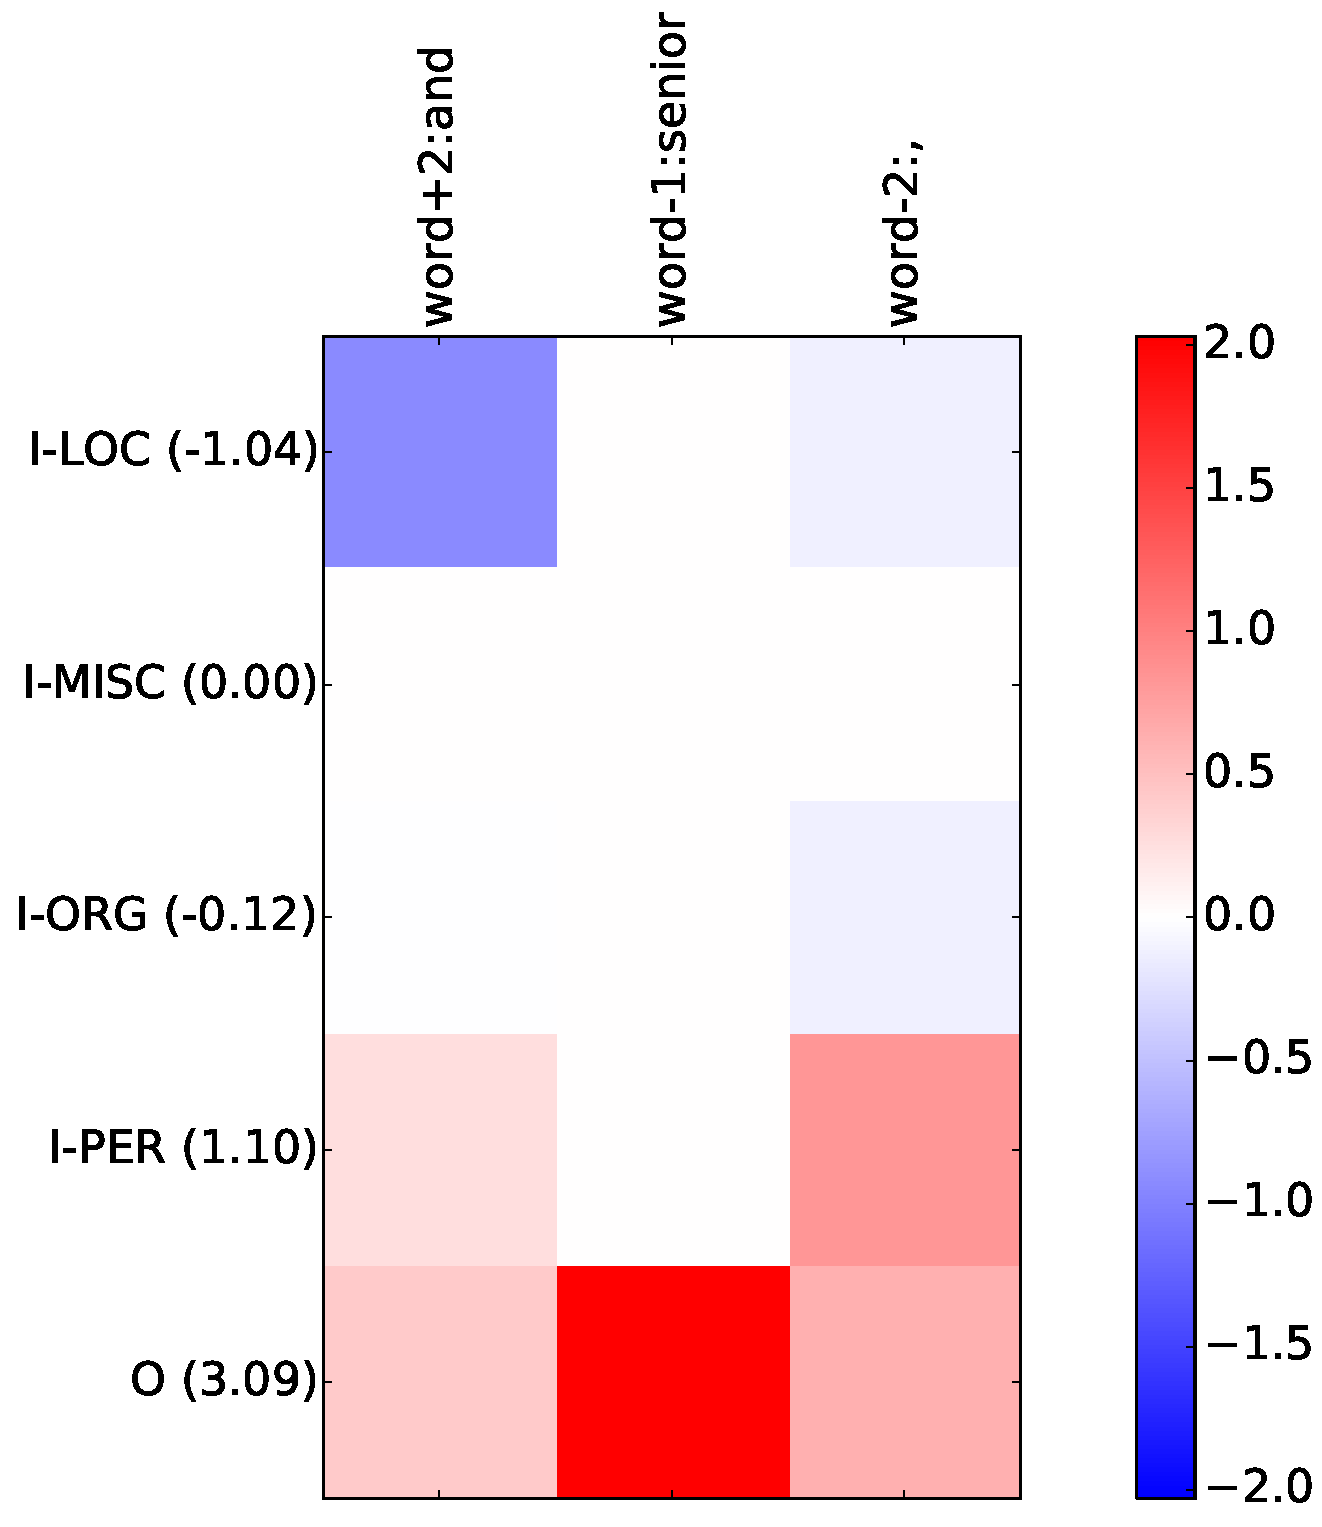
\includegraphics[width=0.9\linewidth]{images/Chapitre4/M1_383.pdf}
	\captionof{figure}{The word \textit{Kory} is predicted to be class O by model $M_1$ given the coefficients of the features indicated.}
	\label{fig:trans_M1}
	\end{subfigure}% 
	\begin{subfigure}[t]{.5\textwidth}
	\centering
	\captionsetup{width=0.7\textwidth}
	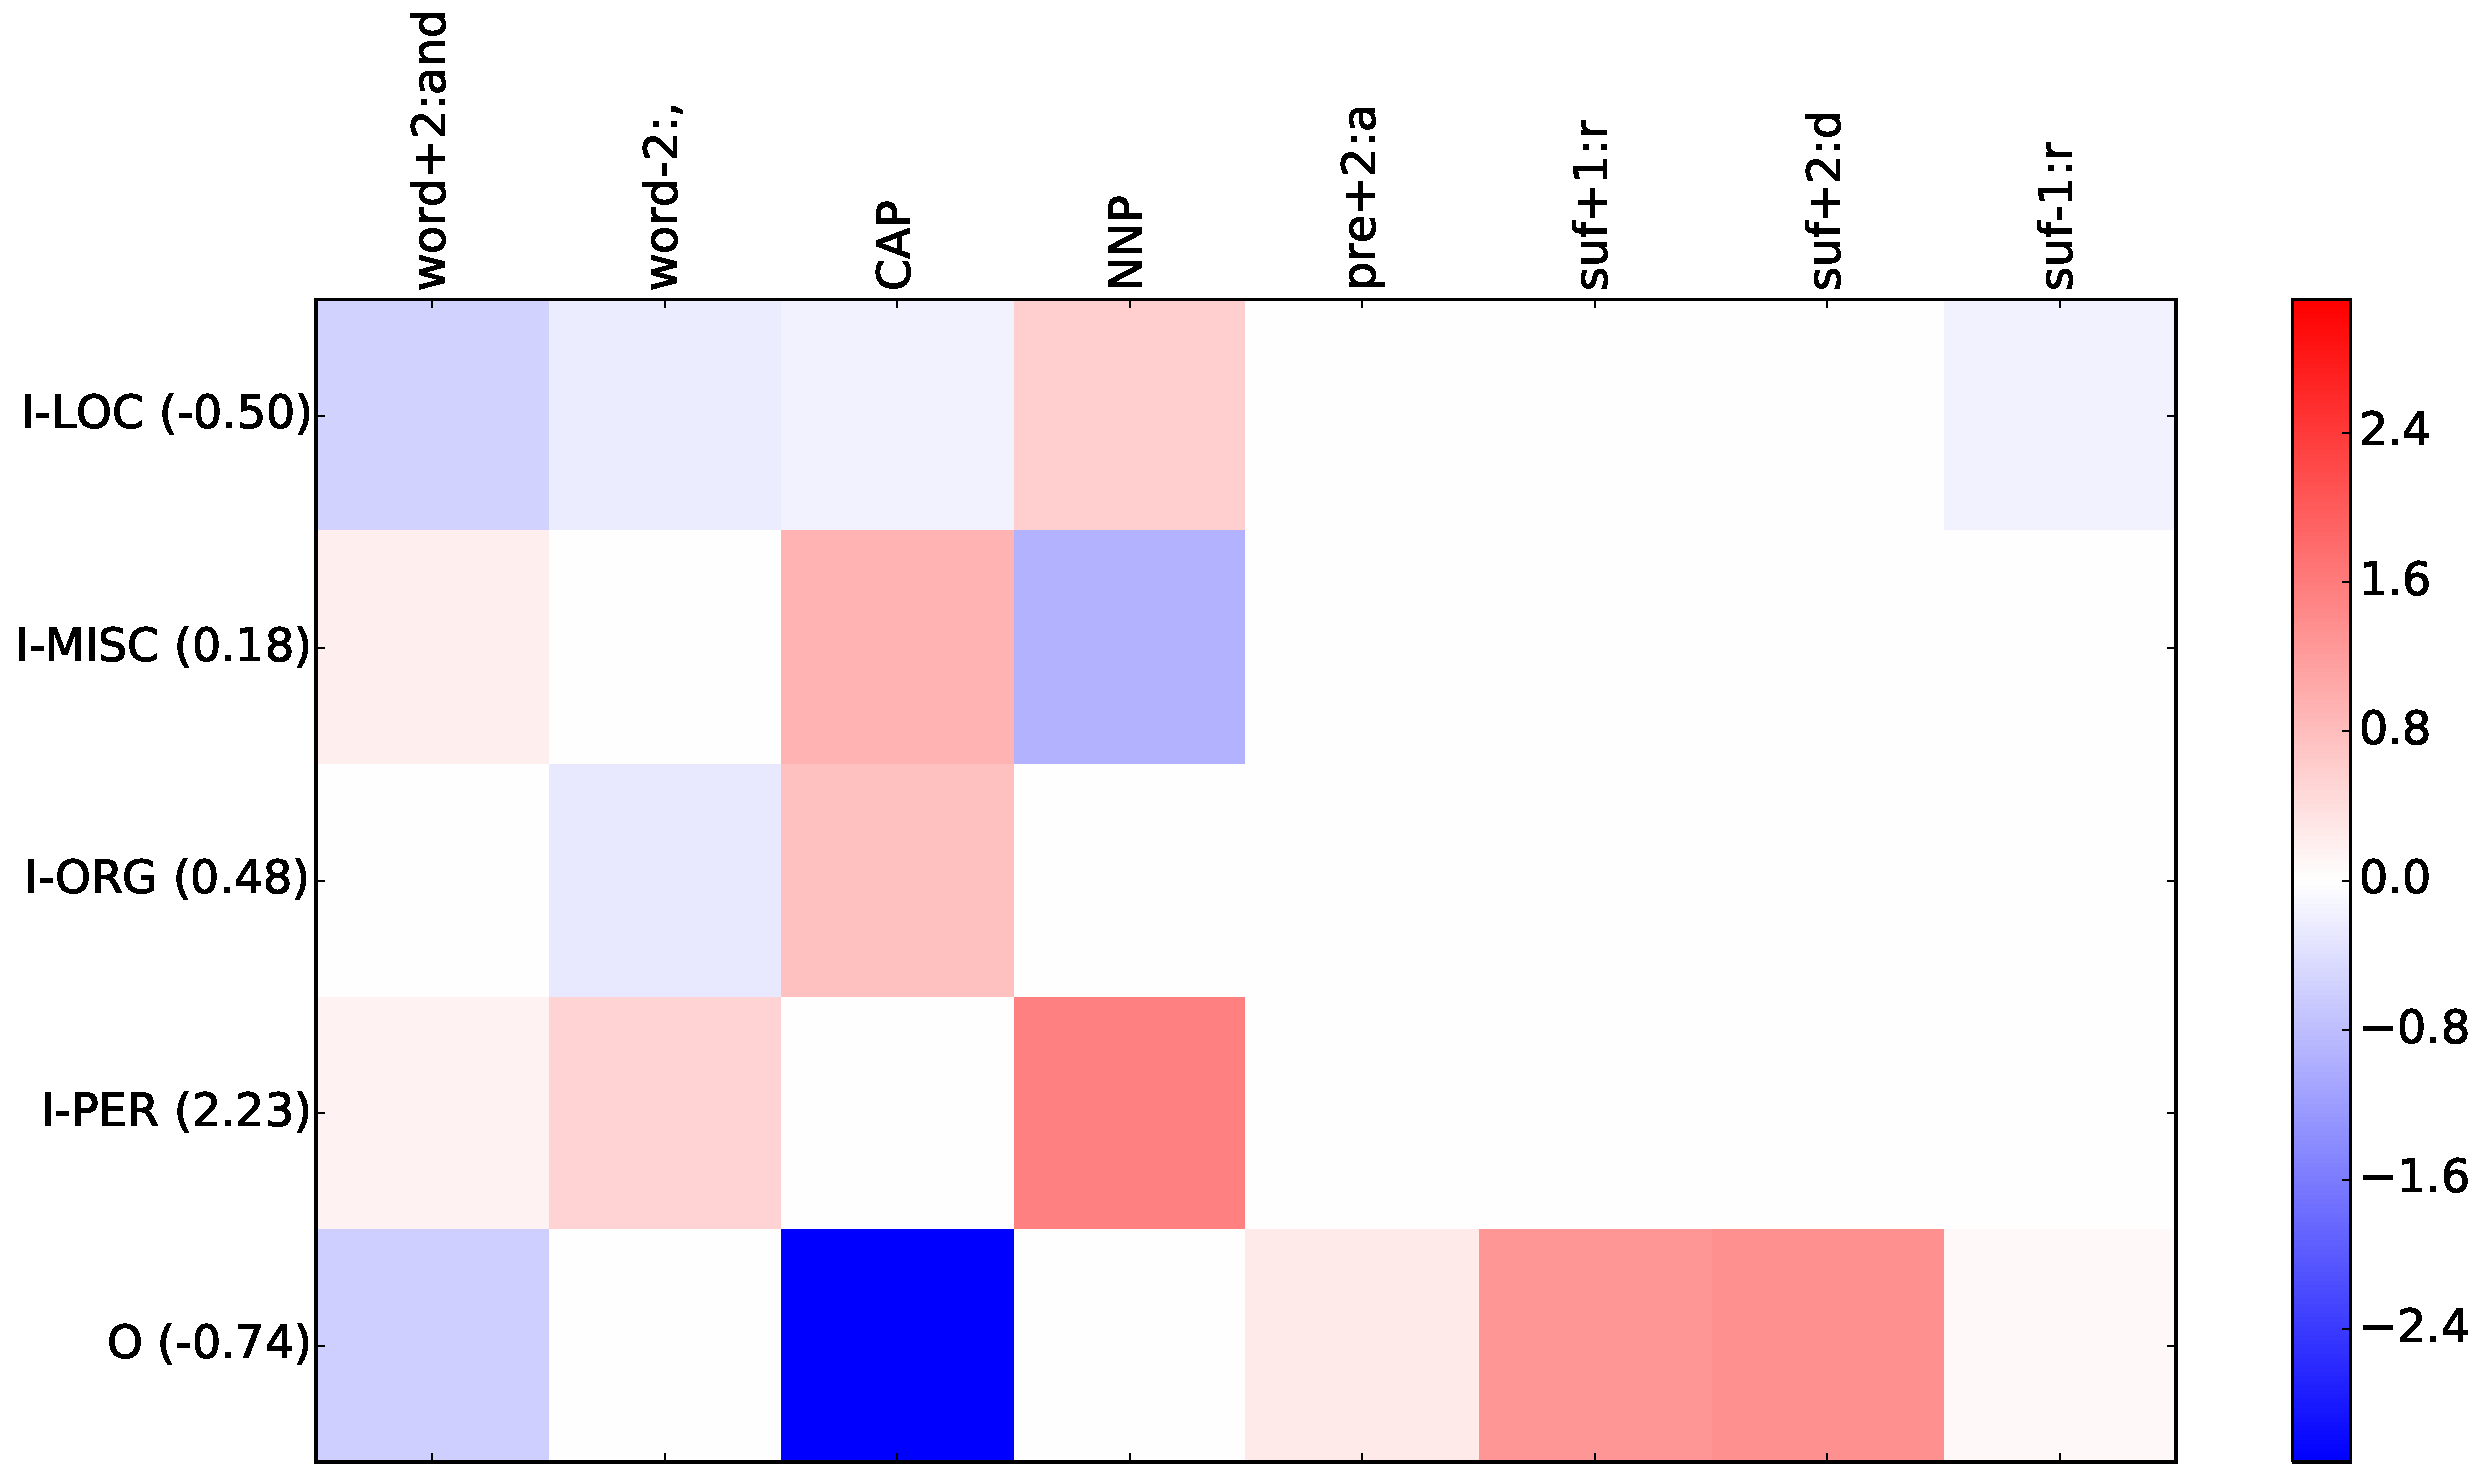
\includegraphics[width=0.9\linewidth]{images/Chapitre4/M2_383.pdf}
	\captionof{figure}{The same word is correctly predicted to be class PER by model $M_2$ given the new features in the model.}
	\label{fig:trans_M2}	
	\end{subfigure}
	\caption{Non-zero coefficients heatmaps for models  $M_1$ and $M_2$ corresponding to the word \textit{Kory}. On the left, $M_1$ fitted using the feature matrix $\mlex$. On the right, model $M_2$ trained using the term $E_{\alpha=0.95}(\mlex, \mstd)$. Red colors are positive, blue are negative. The color intensity varies according to the magnitude of the value.}
	\label{fig:trans_M1_M2}
\end{figure}
\begin{figure}
	\centering
	\begin{subfigure}[t]{.9\textwidth}
	\captionsetup{width=\textwidth}
	\centering
	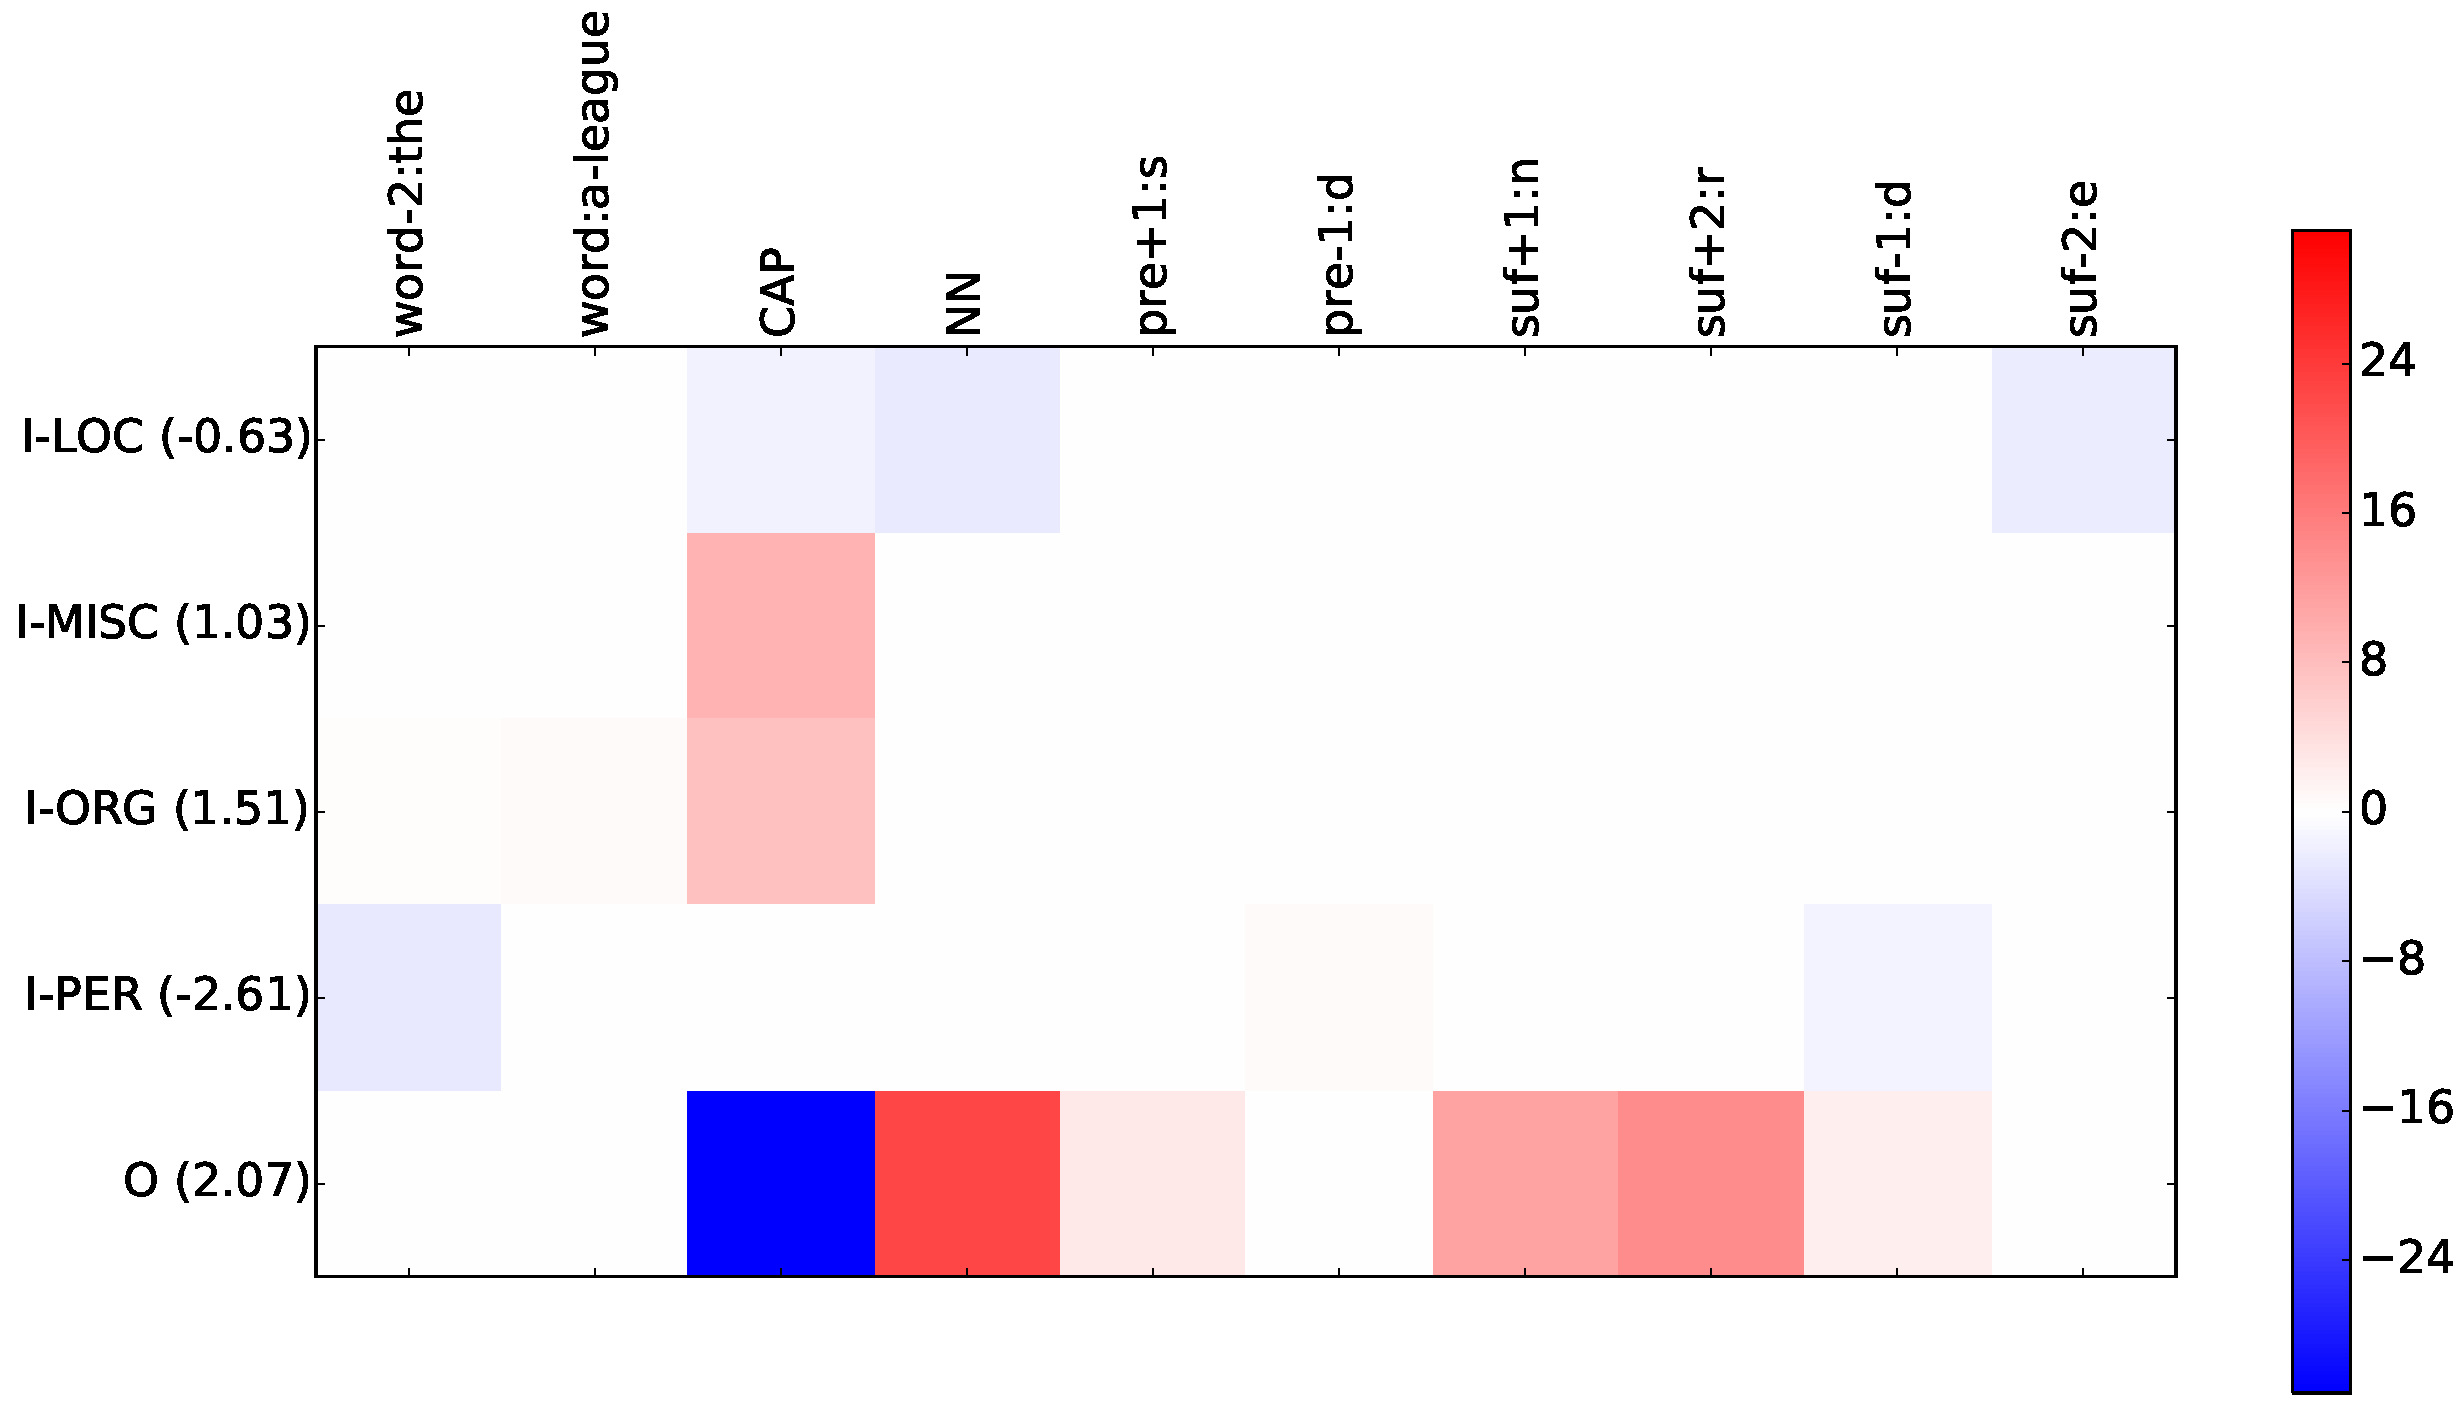
\includegraphics[width=1\linewidth]{images/Chapitre4/M2_1140.pdf}
	\captionof{figure}{The word \textit{A-League} is predicted to be class O by model $M_2$ given the coefficients of the features indicated.}
	\label{fig:trans_M22}
	\end{subfigure}\\%  
	\begin{subfigure}[t]{.9\textwidth}
	\captionsetup{width=\textwidth}
	\centering
	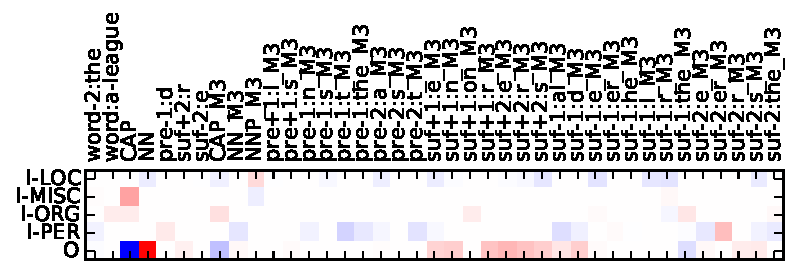
\includegraphics[width=1\linewidth]{images/Chapitre4/M3_1140.pdf}
	\captionof{figure}{The same word is correctly predicted to be class ORG by model $M_3$ given the new features in the model.}
	\label{fig:trans_M3}
	\end{subfigure}
	\caption{Non-zero coefficients heatmaps   for models $M_2$ and $M_3$ corresponding to the word \textit{A-League}. On top, $M_2$ fitted using the term $E_{\alpha=0.95}(\mlex, \mstd)$. On the bottom, model  $M_2$ trained using the  $E_{\alpha=0.95}(\mlex, \mstd, L(\mstd, X_F(\ssyn, \mstd)))$ combination. Red colors are positive, blue are negative. The color intensity varies according to the magnitude of the value.}
	\label{fig:trans_M2_M3}
\end{figure}



\subparagraph{From $\mathbf{M_2}$ to $\mathbf{M_3}$} Going from model ${M_2}$ to ${M_3}$, we focus on the word \textit{A-League}. In the first model, $M_3$ (Figure \ref{fig:trans_M22}), \textit{A-League} is classified as O, since it being a  noun\footnote{The PoS tagger identified it as a simple noun.} (and not a proper noun) seems to be a good indication of a noun not being part of named entity, among other features, such as \textit{suf+2:r}, i.e., the last letter of the second word to the right of \textit{A-League}, in this case \textit{r}. 

With respect to model $M_3$ (see Figure \ref{fig:trans_M3}), \textit{A-League} is correctly tagged as ORG. While the largest coefficients are assigned to the features of the model $M2$ (namely CAP and NN), we can see that the enriched features \textit{CAP\_M3}\footnote{Features added by the third fusion operation are labeled with a \textit{\_M3} suffix. The same is done for the fourth fusion with the suffix \textit{\_M4}} and \textit{suf-1:the\_M3} play a decisive role into the assignation of the class ORG, as most of the values corresponding to the newly added features are positive for this class.



\begin{figure}[h!]
	\centering
	\begin{subfigure}[t]{.9\textwidth}
	\centering
	\captionsetup{width=\textwidth}
	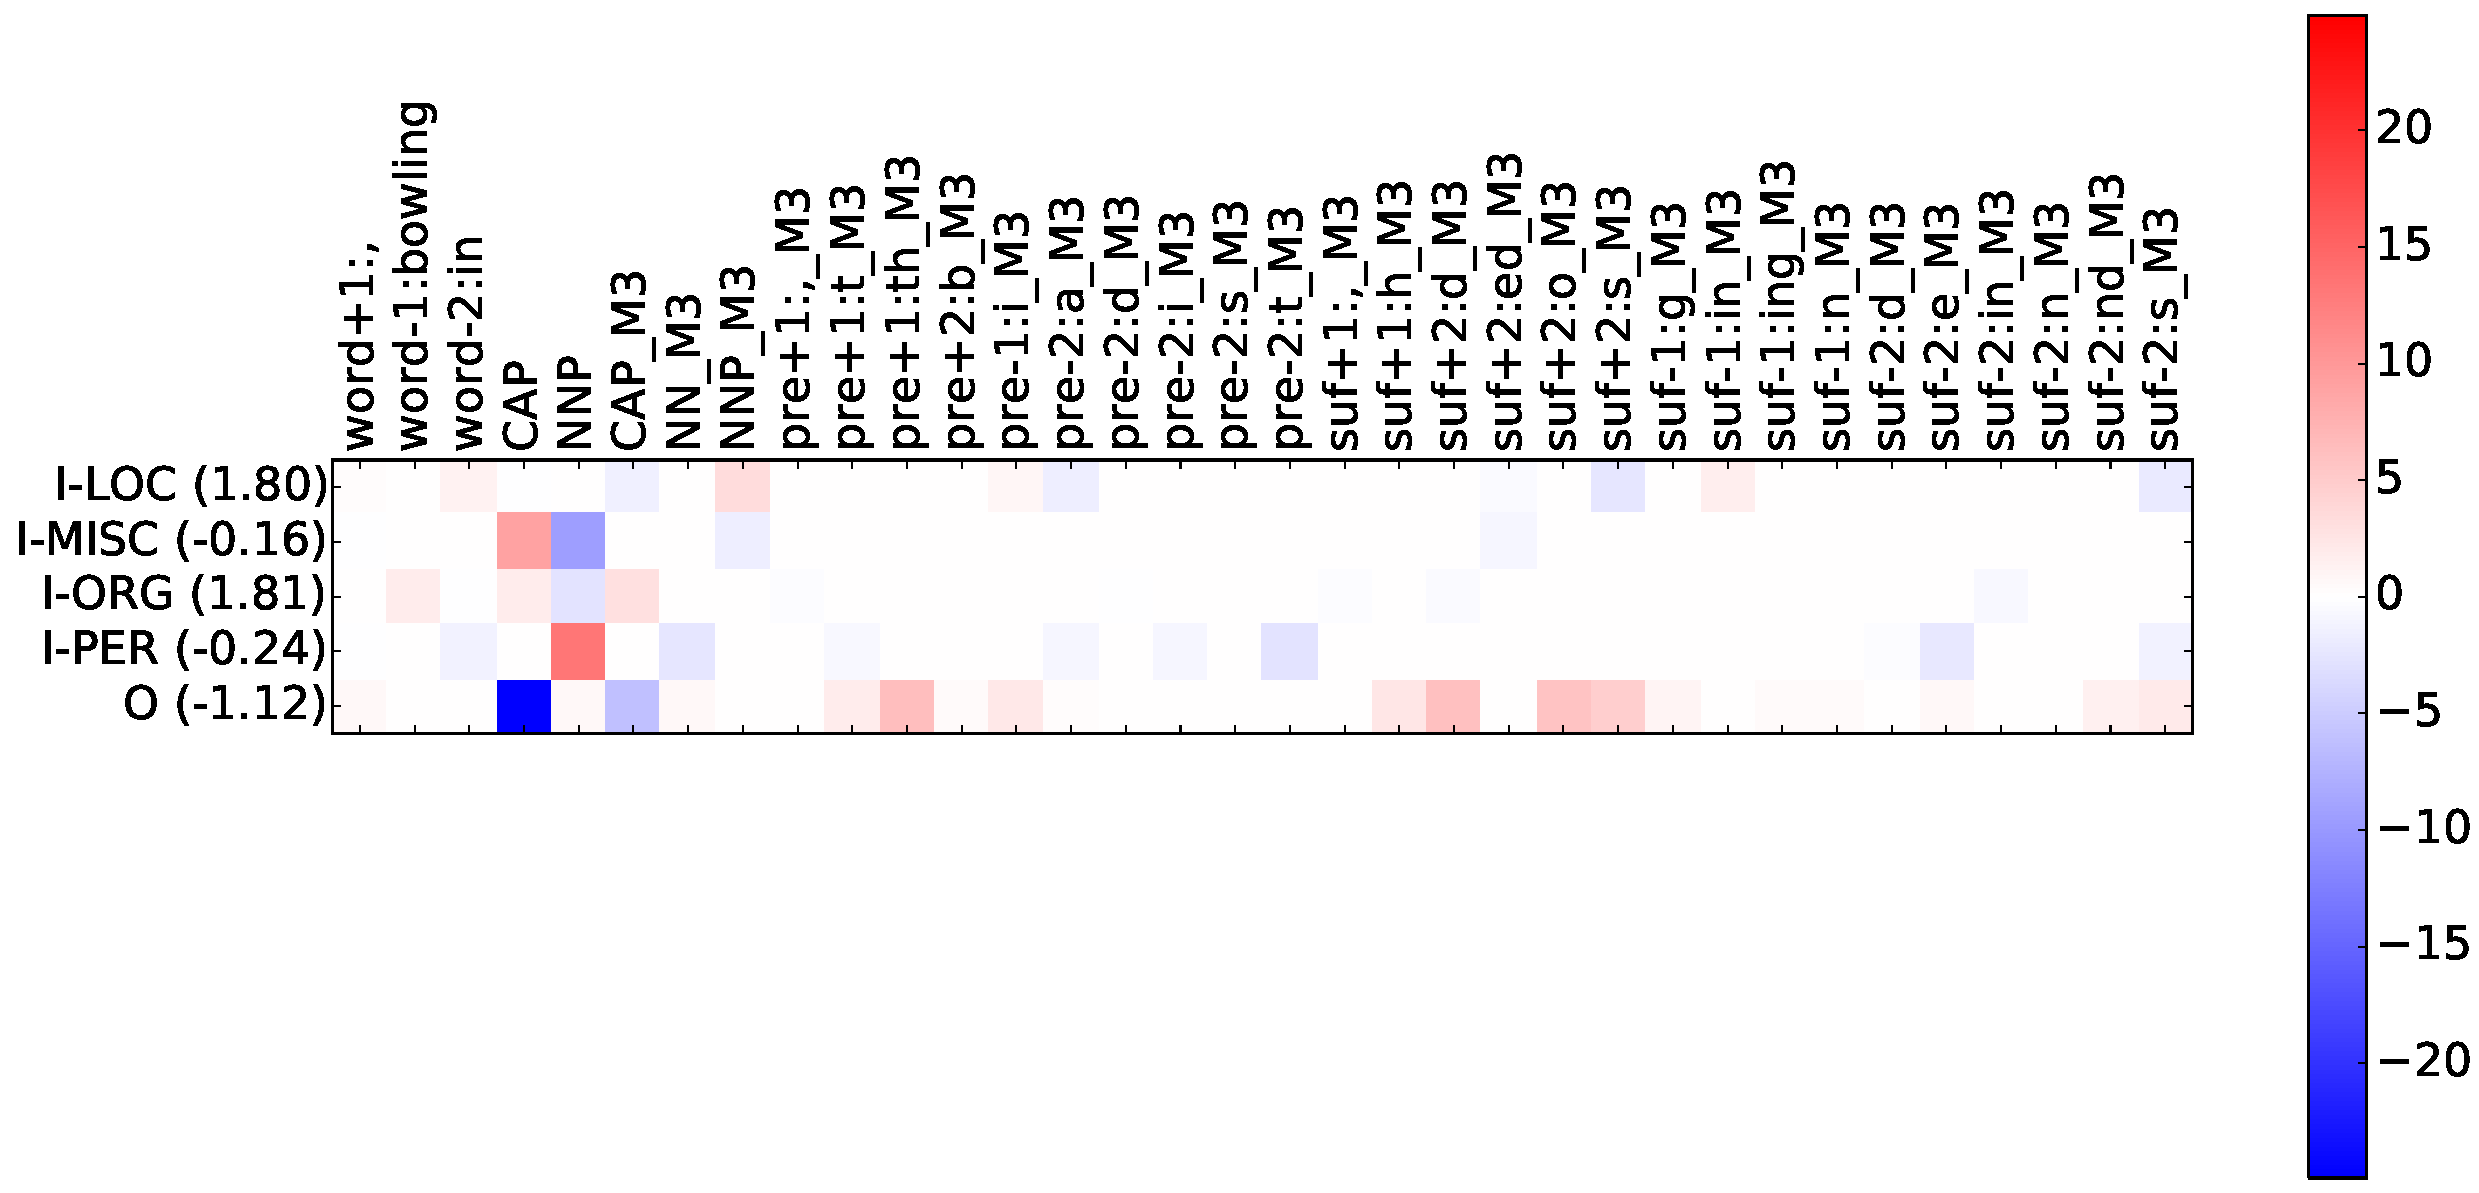
\includegraphics[width=1\linewidth]{images/Chapitre4/M3_16029.pdf}
	\captionof{figure}{The word \textit{Green} is predicted to be class ORG by model $M_3$ given the coefficients of the features indicated.}
	\label{fig:trans_M33}
	\end{subfigure}\\% 
	\begin{subfigure}[t]{.9\textwidth}
	\centering
	\captionsetup{width=\textwidth}	
	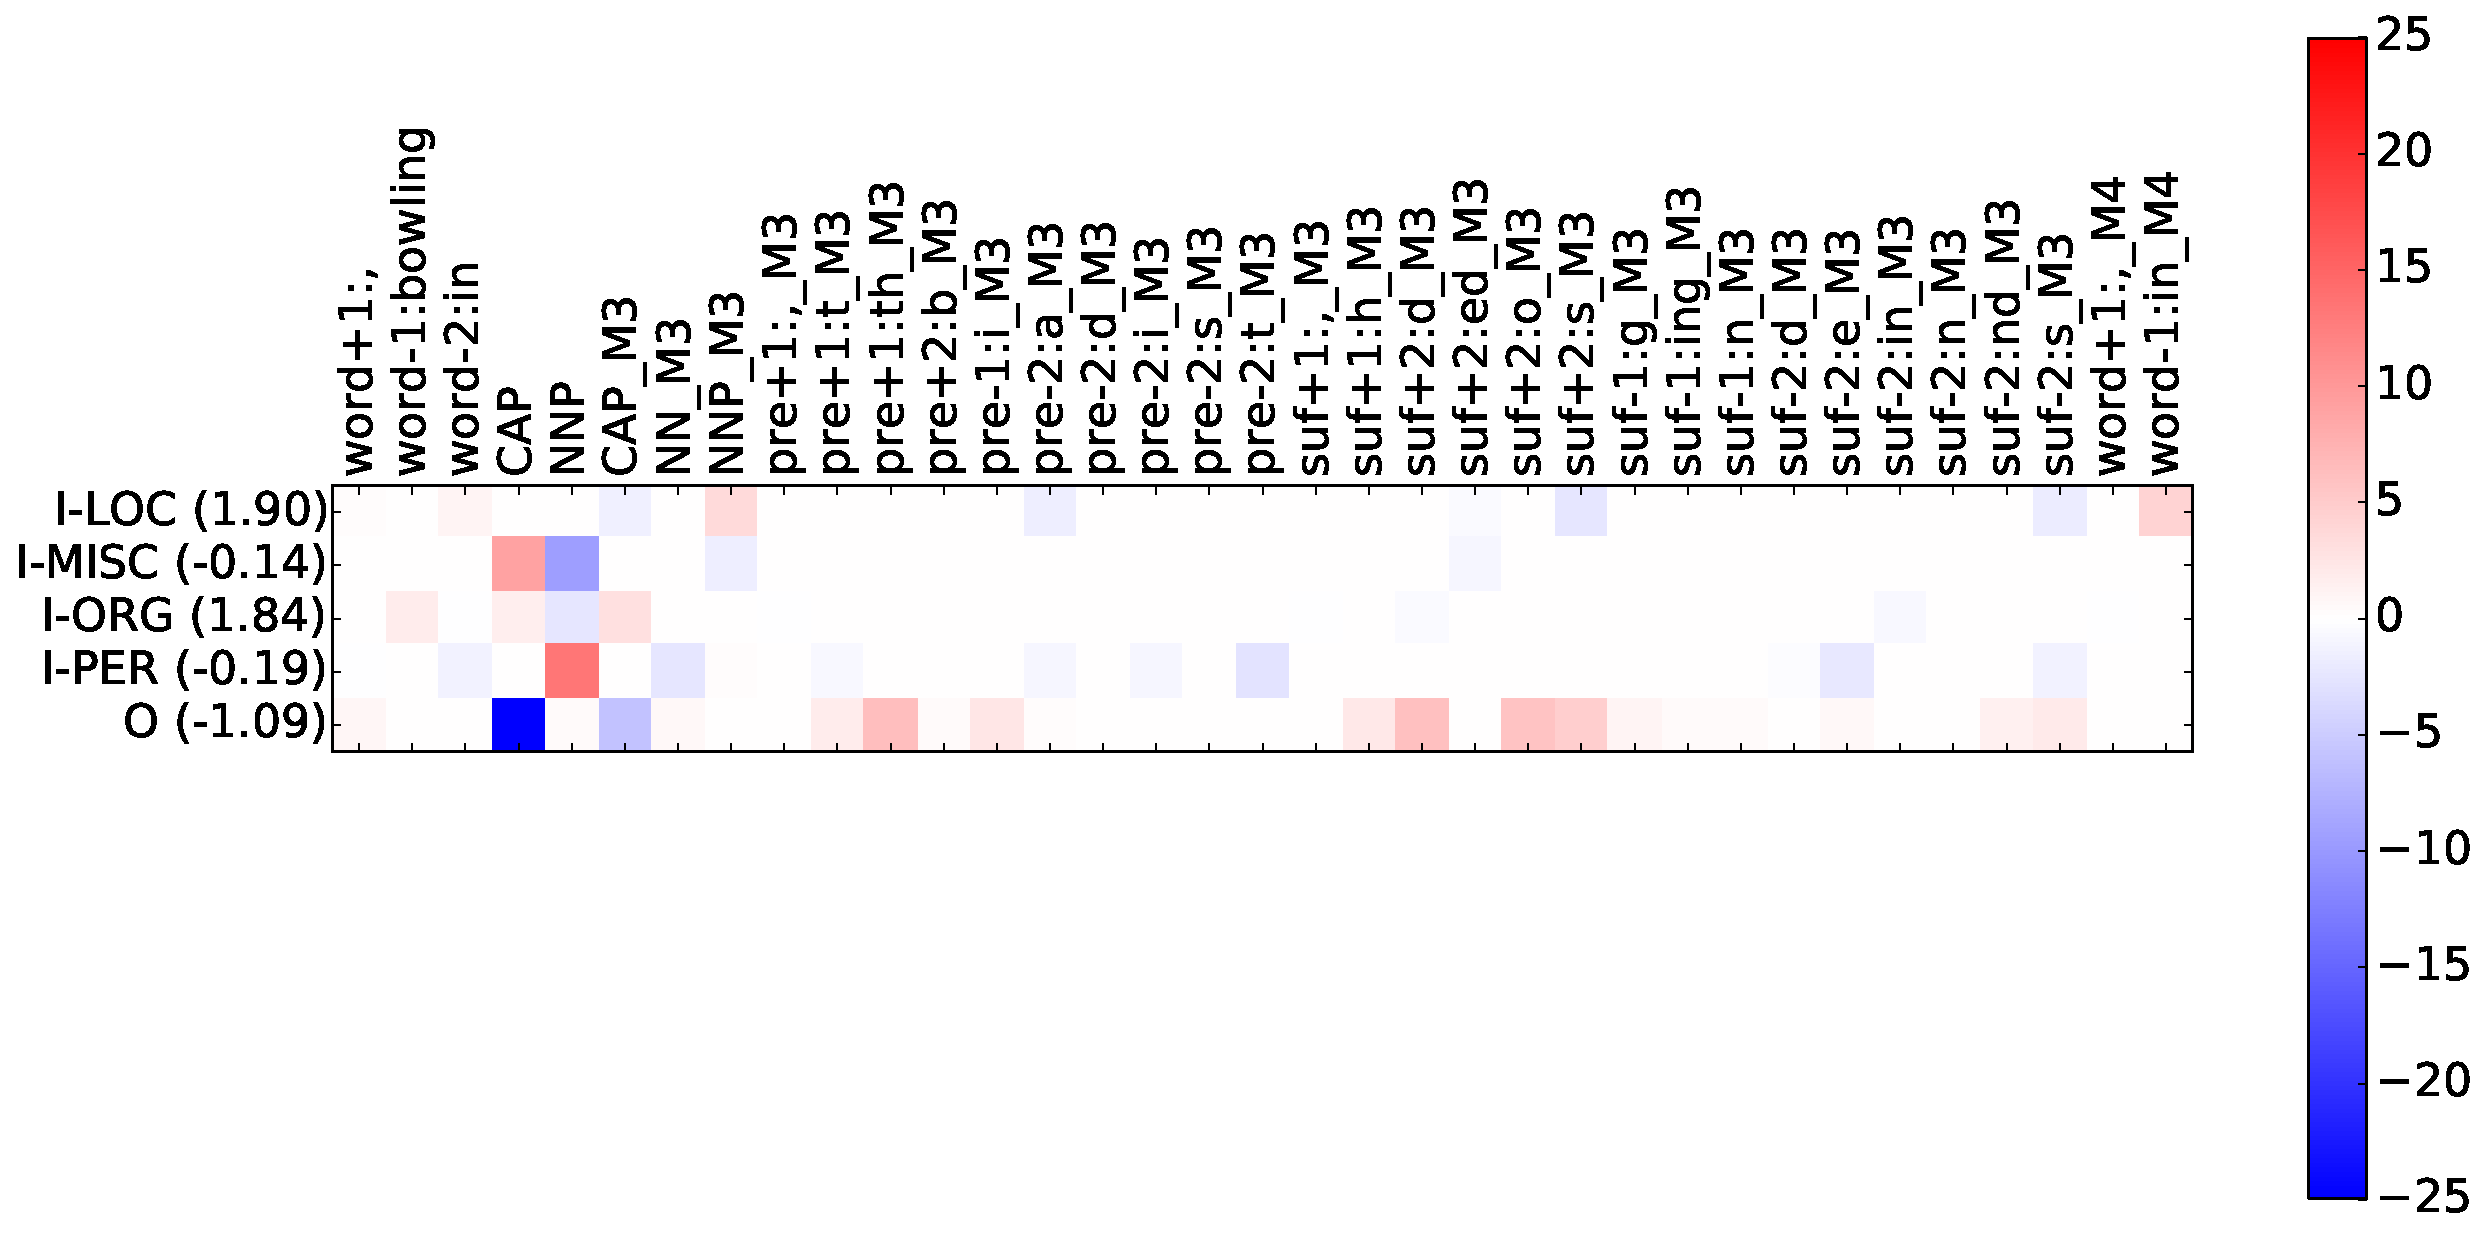
\includegraphics[width=1\linewidth]{images/Chapitre4/M4_16029.pdf}
	\captionof{figure}{The same word is correctly predicted to be class LOC by model $M_4$ given the new features in the model.}
	\label{fig:trans_M4}
	\end{subfigure}
	\caption{Non-zero coefficients heatmaps for  models $M_3$ and $M_4$ corresponding to the word \textit{Green}. On top, $M_3$ fitted using the term $E_{\alpha=0.95}(\mlex, \mstd, L(\mstd, X_F(\ssyn, \mstd)))$. On the bottom, model $M_4$ trained using   $E_{\alpha=0.95}(\mlex, \mstd, L(\mstd, X_F(\ssyn, \mstd)), L(\mlex, X_F(\ssyn, \mlex)))$ as fusion operator. Red colors are positive, blue are negative. The color intensity varies according to the magnitude of the value.}
	\label{fig:trans_M3_M4}
\end{figure}

\subparagraph{From $\mathbf{M_3}$ to $\mathbf{M_4}$} Finally, going from model $M_3 $ to model $M_4$, in Figure \ref{fig:trans_M3_M4} we have an incorrect ORG classification to a correct LOC classification after the application of the last fusion operation. The chosen word is \textit{Green}. Both coefficients' values are quite similar  to each other (see Figures \ref{fig:trans_M33} and \ref{fig:trans_M4}). In fact, the score in parentheses for both LOC and ORG are quite close in both models. This is expected as their difference in performance is small (see Table \ref{tab:4ops}). Not surprisingly, there are only two features coming from the last fusion (the last two columns, indicated with a \textit{\_M4} suffix. Nonetheless, it seems that one of these enriched features, \textit{word-1:in\_M4} determines the model decision towards the LOC class, thus making the correct classification.

In general, in these experiments, we see that the added enriched features are not the highest valued in the fitted coefficients vectors, nonetheless, they  provide the extra information needed to push the model towards the correct prediction, by enriching the features through cross and late fusion and by providing more descriptors for each word and consequently reducing the sparsity of the representation matrices.

Once we found a set of fusion operations that work reasonably well with NER, we experiment with another task, word sense induction and disambiguation, to confirm the usefulness of using fusion enriched representations to train better models.

In the next subsection we present a series of analogous experiments, this time solving WSI/WSD.


\section{Second Application: Word Sense Induction and Disambiguation}
\label{sec:wsd_wsi}
Word Sense Induction and Disambiguation entails two closely related tasks\footnote{Even though these tasks are closely related, they are independent from one another. Still,  we consider them to be a single one: WSI/WSD.}. WSI aims to automatically discover the set of possible senses for a target word given a text corpus containing several occurrences of said target word. Meanwhile, WSD takes a set of possible senses and determines the most appropriate sense for each instance of the target word according to the instance's context. WSI is usually approached as an unsupervised learning task, i.e., a cluster method is applied to the words occurring in the instances of a target word. The groups found are interpreted as the senses of the target word. The WSD task is usually solved with knowledge-based approaches, based on WordNet; or more recently with supervised models which require annotated data. It can be also solved reasonably well by comparing the words surrounding each target word and the words belonging to the induced senses (or clusters) found during the WSI step.

We believe that in order to solve WSD in a truly end-to-end unsupervised way, one would need to first automatically find a list of senses for a word without the help of pre-built semantic networks. In other words, solve WSI. Word sense induction is usually solved as follows:

Given an input document with a set of target words, coupled with a set of contexts (a target word in a unique context is called an instance), the goal is to discover a list of senses for each target word and then assign each instance in the document with an automatically generated sense (this part corresponds to WSD). The common four steps used are the following:

\begin{enumerate}
\item Build a lexical co-occurrence network (LCN), or similar, assigning tokens as nodes and  establishing edges between them if they co-occur in a given context (usually if they both appear in the same sentence, paragraph or fixed window of words).
\item Determine the weights for each edge either according to a frequency metric or using binary weights. 
\item Apply a graph clustering algorithm. Each cluster found will represent a sense of the polysemous target word.
\item Match target word instances with the clusters found (the senses) by using the word context. Specifically, assign a sense to each instance by looking at the tokens in the context. This step is actually the word sense disambiguation task. 
\end{enumerate}	


Word sense induction, while being an unsupervised and thus more flexible task (language and word-domain independent, does not require human-made knowledge bases), require a good quality clustering algorithm, as its results are tightly linked to its performance.
\subsection{Fusion Enriched Representations}

In this subsection we also employ the hypergraph model introduced before to propose a solution to both WSD and WSI tasks, specifically the enrichment of features via fusion techniques.

The WSI method, i.e., the clustering algorithm, we employ is not original, as we will see. Nonetheless, our interest lies on  using a combined representation, which is able to address certain concerns that are not deeply studied, namely the use of heterogeneous context features to solve semantic tasks while reducing the number of parameters compared to similar approaches.  Our method is evaluated with a corpus corresponding to the WSI task of the international workshop of semantic evaluations, edition 2007, or Semeval 2007. 

As shown in Figure \ref{fig:diagmetodoWSD}, the procedure we follow is very similar to that of the previous NER experiments. The difference being the task addressed and the features employed (we find clusters using only lexical and syntactic contexts).
\begin{figure}[t]
\centering
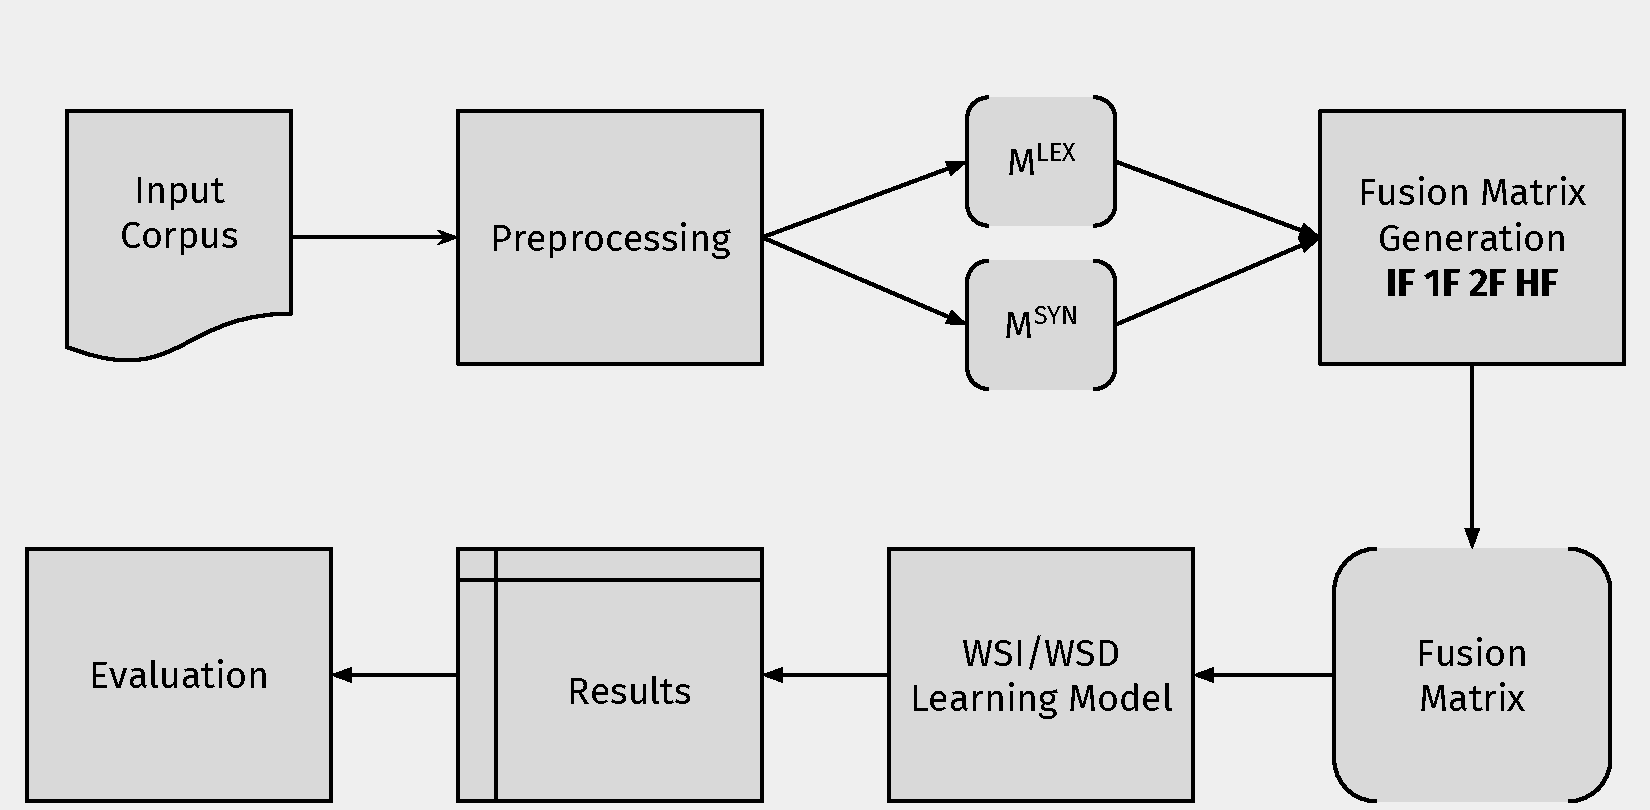
\includegraphics[width=0.85\linewidth]{images/Chapitre4/diag_metodoWSD.pdf}
\caption{Steps followed on our fusion-enriched representation for WSI/WSD experiments. First the corpus is lightly preprocessed, then features are extracted from the text. A fusion matrix is generated, which in turn is used as input to the learning algorithm. Finally, the system yields its results and to be analyzed.}
\label{fig:diagmetodoWSD}
\end{figure}
%\subsection{Introduction}



We discovered a set of successful fusion operations in the previous experiments. In these experiments we set to test if the improvements obtained before, using said fusion schemes, can be transferred into WSI/WSD and other corpora. 

\paragraph{Representation Spaces}
We use the same set of features from the previous subsection (see \ref{sec:rep_spaces}), except for the standard NER features, that is, those represented by $\mstd$, as they are specifically designed to tackle that task. Consequently, we will experiment with two representation matrices $\mlex$ and $\msyn$.

\paragraph{Learning Methods}
Regarding the machine learning methods to induce senses, (the WSI part), we employ spectral clustering (as is described previously in Chapter 3, paragraph \ref{par:partitioning_clustering}) on the input matrices in order to automatically discover senses (a cluster is considered a sense). As we noted before, this method require as input a symmetric positive similarity matrix. Given that our fusion operators already may yield similarity matrices (e.g., late fusion of similarity matrices). If that is the case, we use this type of matrix directly as input to the algorithm. Otherwise, we compute the cosine similarity to obtain the corresponding affinity matrix and then use it as input. Similarly, spectral clustering is said to be more efficient if the input matrix is sparse \cite{song2008parallel}. We do not sparsify the matrix, usually done by applying a top-$k$ nearest neighbors selection, as we already apply said selection in certain fusion operators and it then becomes even harder to track the modifications applied to the feature space.

 Regarding disambiguation, we trivially assign senses to the target word instances according to the number of common words in each cluster and the context words of the target word. In other words, for each test instance of a target word, we select the cluster (sense) with the maximum number of shared words with the current instance context.

\paragraph{Experiments and Evaluation}
Having learned the best fusion configuration from the previous task, in these experiments we set to test if the improvements achieved can be transfered into another NLP task, namely Word Sensed Induction and Disambiguation (WSI/WSD). As preprocessing, we simply remove stopwords and tokens with less than three letters. The features we extracted from the tested corpora with the same tools as in the previous task.
\subparagraph{Test Dataset}
The WSI/WSD model is tested on the dataset of  the Semeval 2007 WSID task \cite{Agirre2007}. The task was based on a set of 100 target words (65 verbs and 35 nouns), each  word having a set of instances, which are specific contexts where the word appear. Senses are induced from these contexts and applied to each one of the instances. The real number of average senses per word is 2.87 in the test set, which was the set used to evaluate the competing systems. This number will be useful to determine the performance of the systems below.



\subparagraph{Evaluation Measures}
Being an unsupervised task, the evaluation metrics of WSI/WSD are debated in terms of quality \cite{CruysA11}. We consider supervised recall and unsupervised F-measure, as in the competition original paper \cite{Agirre2007}. 

Ihe unsupervised evaluation assumed the induced senses as clusters of examples. These clusters are compared to the sets of examples tagged with the given gold standard word senses (classes), and evaluated using the F-measure measure for clusters. The supervised setting maps the induced senses to manually-defined gold standard senses, and use a mapping produced by the organizers to tag the test corpus with gold standard tags. The mapping is automatically produced by the organizers, and the resulting results evaluated according to the usual precision and recall measures for supervised word sense disambiguation systems. 

%The first one maps the output of a system to the true senses of the target words' instances and the second one measures the quality of the correspondence between the automatically found clusters and the senses. 

We consider that the number of senses found by the system is also a rather good indicator of performance: the best competition baseline assigns the Most Frequent Sense baseline (or MFS) to each test instance of each target word. In other words, each test instance is assigned the sense that occurs the most in the training set. Consequently, this baseline produces an average of one sense (cluster) per word. A system that goes near this average may be indeed not be resolving the task efficiently but finding the one cluster per word trivial solution. Consequently, to show that we do not fall in the MFS solution, we display in our results the average number of clusters. Furthermore, given this problematic situation we introduce a simple measure, the H-measure, that takes into account three factors of the performance results of a system: the supervised recall of all-words ($SR$), the unsupervised F-measure of all-words ($UF$), and the number of true senses on the corpus. The H-measure is calculated as the mean of two components. First, the harmonic mean of the $SR$ and the $UF$. Secondly, a ratio we propose that is bounded between zero and one. Zero indicates that the system produces one cluster per word, that is, the baseline. If the ratio is one, the system produces a number of average cluster per word that is close to the true gold-standard average number of senses. We call this quantity $\delta$. More formally, the H-measure is defined as:

\begin{equation}
\text{H-measure} = \dfrac{1}{2}\left(2*\dfrac{SR*UF}{SR+UF}+\dfrac{\delta}{\delta+|\#cl-\delta|}\right)
\end{equation}

This metric is bounded between 0 and 1 as the F-measure and recall. The greater its value, the more confidently we  say that the system produces good results. The way it is formulated, having the F-measure and the recall within the formulation serves as an assurance against having systems that are bad but coincidentally produces a correct number of senses. Given that we are calculating the harmonic mean of another harmonic mean (within the F-measure) makes the H-measure severe regarding F-measure and recall. Improvements on both metrics must be had to show a growth in  the H-measure.

We consider this measure as a simple method to rank the results that follow, as the metrics provided by the WSI/WSD competitions are not always ideal and have their own issues, and more importantly, because they may contradict each other. Still, the H-measure is not intended to replace the classic metrics. 


\begin{table}[htp!]
\centering
%\setlength\tabcolsep{3pt}
\caption{All-words, nouns, and verbs supervised recall for the Semeval 2007 corpus using fusion operations (SF, 1F, 2F, HF) and spectral clustering. We also display the average number of clusters found by each fusion configuration, the best performing system as well as the MFS baseline. In bold the best results per-column among our experiments.}
\label{tab:wsd-semeval_sup_Recall}
\begin{tabular}{@{}lrrrrc@{}}
\toprule
\textbf{Fusion Operation / System} & \multicolumn{3}{c}{\textbf{Recall (\%)}} & \#\textbf{cl} & \textbf{Fusion Level}\\ 
        & \textbf{all}          & \textbf{nouns}          & \textbf{verbs} &          \\ 
       \midrule
        \multicolumn{5}{r}{\textbf{Single Features}} & \multirow{3}{*}{\textbf{SF}} \\ %\midrule
       $\mlex$                    & 79.20 & 82.10 & 75.80 & 4.13\\
 

       $\msyn$                    & 79.10 & 81.60 & \textbf{76.20} & 4.47\\
       \midrule
                   \multicolumn{5}{r}{\textbf{Early Fusion (EF)}}  & \multirow{10}{*}{\textbf{1F}}     \\ %\midrule
       $E(\mlex, \msyn)$		& 78.70 & 81.11 & 76.10 & 4.46\\
	  %\midrule
                   \multicolumn{5}{r}{\textbf{Cross Feature Fusion ($\mathbf{X_FF}$)}}       \\ %\midrule	         
	   
	   $X_F(\slex, \mlex)$		& 79.20 & 82.30 & 75.70  & 3.63\\	   
       $X_F(\slex, \msyn)$		& 78.30 & 80.90 & 75.30  & 3.08\\
	   $X_F(\ssyn, \mlex)$		& 78.60 & 80.90 & 76.10  & 1.08\\	   
       $X_F(\ssyn, \msyn)$		& 78.90 & 81.40 & 76.10 & 2.72\\       
 %\midrule
                   \multicolumn{5}{r}{\textbf{Cross Similarity Fusion ($\mathbf{X_SF}$)}}       \\ %\midrule
	   
 
	   $X_S(\ssyn, \slex)$		& 78.70 & 80.90 & \textbf{76.20}  & 1.01\\
	   $X_S(\slex, \ssyn)$		& 78.80 & 80.90	& 76.06 & 1.33\\
	  
 \midrule
                   \multicolumn{5}{r}{\textbf{Cross Feature Cross Similarity Fusion ($\mathbf{X_FX_SF}$)}}  & \multirow{9}{*}{\textbf{2F}}     \\ %\midrule
	   
       $X_F(X_S(\slex, \ssyn), \mlex)$		& 78.40 & 80.40 & 76.10 & 3.11 \\	   
       $X_F(X_S(\slex, \ssyn), \msyn)$		& 78.90 & 81.80 & 75.60 & 3.16\\	   
       	  %\midrule
                   \multicolumn{5}{r}{\textbf{Early Cross Feature Fusion ($\mathbf{EX_FF}$)}}       \\ %\midrule	         
       
       $E(\mlex, X_F(\slex, \mlex))$		& 79.20 & 82.40 & 75.70 & 3.57\\	   
	   $E(\msyn, X_F(\slex, \mlex))$		& 78.30 & 80.50 & 75.80 & 1.95\\	   
       %\midrule
                   \multicolumn{5}{r}{\textbf{Late Cross Feature Fusion ($\mathbf{LX_FF}$)}}       \\ %\midrule	  
	   $L(\msyn, X_F(\slex, \msyn))$		& 78.60 & 81.10 & 75.80 & 4.22\\	   
	   $L(\mlex, X_F(\slex, \mlex))$		& \textbf{79.50} & \textbf{82.80} & 75.70 & 3.96\\	   
       \midrule
                   \multicolumn{5}{r}{\textbf{Early Late Cross Feature Fusion ($\mathbf{ELX_FF}$)}}     & \multirow{3}{*}{\textbf{HF}}  \\ %\midrule	  
	   $E(\mlex, L(\msyn, X_F(\slex, \msyn)))$		& 78.50 & 81.40 & 75.40 & 4.26\\	   
	   $E(\mlex, L(\mlex, X_F(\slex, \mlex)))$		& \textbf{79.50} & 82.70 & 75.90 & 3.99\\
	   \midrule
	   \midrule
	   

	   Baseline MFS		& 78.70 & 80.90 & 76.20 & 1.00\\ 	   	 	    
%	   Semeval 2007 Best System& 81.60 & 86.80 & 75.70 & 1.15\\ 	 		   
       \bottomrule
\end{tabular}
\end{table}


\begin{table}[htp!]
\centering
\setlength\tabcolsep{3pt}
\caption{All-words, nouns, and verbs unsupervised F-measure for the Semeval 2007 corpus using fusion operations (SF, 1F, 2F, HF) and spectral clustering. We also display the average number of clusters found by each fusion configuration, the best performing system as well as the MFS baseline. In bold the best results per-column among our experiments.}
\label{tab:wsd-semeval_unsup_fm}
\begin{tabular}{@{}lrrrrc@{}}
\toprule
\textbf{Fusion Operation / System} & \multicolumn{3}{c}{\textbf{F-measure (\%)}} & \#\textbf{cl} & \textbf{Fusion Level}\\ \midrule
      	& \textbf{all}          & \textbf{nouns}          & \textbf{verbs}           \\ 
       \midrule
       \multicolumn{5}{r}{\textbf{Single Features}} & \multirow{3}{*}{\textbf{SF}}\\ %\midrule
       $\mlex$                    &	72.70	 & 76.90 & 67.90 & 4.13\\
 

       $\msyn$                    &	69.30	& 69.40 & 69.20 & 4.47\\
       \midrule
       \multicolumn{5}{r}{\textbf{Early Fusion (EF)}}  & \multirow{10}{*}{\textbf{1F}}     \\ %\midrule
       $E(\mlex, \msyn)$		&	74.00	& 76.66 & 71.11 & 4.46\\
	  %\midrule
       \multicolumn{5}{r}{\textbf{Cross Feature Fusion ($\mathbf{X_FF}$)}}       \\ %\midrule	         
	   
	   $X_F(\slex, \mlex)$		&	76.20	& 79.60 & 72.50 & 3.63 \\	   
       $X_F(\slex, \msyn)$		&	74.60	& 75.10 & 73.90 & 3.08 \\
	   $X_F(\ssyn, \mlex)$		&	\textbf{78.90}	& 80.70 & \textbf{76.90}	 & 1.08 \\	   
       $X_F(\ssyn, \msyn)$		&	73.70	& 77.70 & 70.00 & 2.72 \\       
% \midrule
       \multicolumn{5}{r}{\textbf{Cross Similarity Fusion ($\mathbf{X_SF}$)}}       \\ %\midrule
	   
 
	   $X_S(\ssyn, \slex)$		&	\textbf{78.90}	& \textbf{80.80} & 76.80 & 1.01 \\
	   $X_S(\slex, \ssyn)$		&	78.70	& 80.50  & 76.80 & 1.33 \\
	  
 \midrule
       \multicolumn{5}{r}{\textbf{Cross Feature Cross Similarity Fusion ($\mathbf{X_FX_SF}$)}}   & \multirow{9}{*}{\textbf{2F}}    \\ %\midrule

       $X_F(X_S(\slex, \ssyn), \mlex)$		&	70.00	&68.70  & 71.40& 3.11 \\	   
       $X_F(X_S(\slex, \ssyn), \msyn)$		&	75.20	& 77.40 & 72.80 & 3.16 \\	   
       	  %\midrule
       \multicolumn{5}{r}{\textbf{Early Cross Feature Fusion ($\mathbf{EX_FF}$)}}       \\ %\midrule	         
       
       $E(\mlex, X_F(\slex, \mlex))$		&	76.00	& 79.50  & 72.10 & 3.57 \\	   
	   $E(\msyn, X_F(\slex, \mlex))$		&	75.20	&75.40  & 75.00 & 1.95 \\	   
       %\midrule
       \multicolumn{5}{r}{\textbf{Late Cross Feature Fusion ($\mathbf{LX_FF}$)}}       \\ %\midrule	  
	   $L(\msyn, X_F(\slex, \msyn))$		&	67.80	& 71.40&63.80 & 4.22 \\	   
	   $L(\mlex, X_F(\slex, \mlex))$		&	76.09	&79.10 &72.70 & 3.96 \\	   
       \midrule
       \multicolumn{5}{r}{\textbf{Early Late Cross Feature Fusion ($\mathbf{ELX_FF	}$)}}    & \multirow{3}{*}{\textbf{HF}}   \\ %\midrule	  
	   $E(\mlex, L(\msyn, X_F(\slex, \msyn)))$		&	74.20	& 78.20 & 69.80& 4.26 \\	   
	   $E(\mlex, L(\mlex, X_F(\slex, \mlex)))$		&	75.80	& 78.50&72.70 & 3.99 \\
	   \midrule
	   \midrule
	   Baseline 1c1word 		&	78.90	& 80.70&76.80 & 1.00 \\ 	   	 	    	   
%	   Semeval 2007 Best Systems	&	78.70	& 80.80&76.30 & 3.06 \\ 	 

		   
       \bottomrule
\end{tabular}
\end{table}




\paragraph{Results and Discussion}
Word sense induction and disambiguation results, using fusion enriched matrices with spectral clustering, are found in Tables \ref{tab:wsd-semeval_sup_Recall} and \ref{tab:wsd-semeval_unsup_fm} for the supervised recall and unsupervised F-measure respectively. We present the results for al words, nouns and verbs. The values corresponding the H-measure are discussed immediately following the analysis of the recall and F-measure.

In the unsupervised evaluation results, we include an interesting baseline which had also the best performing results. The baseline consists in assigning one cluster per word (or {1c1word}), i.e., it simply assigns a single sense to all the test instances of a word. This baseline was not beat during the competition. On the other had, for the supervised results, we include the Most Frequent Sense (or MFS) baseline which tags every test instance with the sense that occurred most often in the training corpus of the competition. Besides these baselines, we included also the best performing systems' results for both of the evaluations.


We experimentally set $\beta=0.90$ and $\gamma=50$. Remember that $\beta$ controls the relevance of each matrix in the late fusion binary operator $L(\beta\cdot A, (1-\beta)\cdot B)$ and $\gamma$ control number of nearest neighbors to take from the first operand of the cross fusion $\mathbf{K}(A,\gamma) \times B$. The parameter $\alpha$ of the early fusion operator is not employed (i.e., we concatenate matrices without weighting them) unless the value of $\alpha$ is explicitly specified.
%Specifically regarding this WSI/WSD task, late fusion, when the first matrix  is deemed more relevant than the second one, the performance is higher. This may be due to the fact that, in this task, the feature matrices rows contain types (that is, each line represent an unique word), and thus they are more dense, which may entail more noisy data. By reducing the relevance of the second matrix in late fusion, we are effectively attenuating the less important information.

%Concerning the parameter $\gamma=50$ in cross fusion (remember that $\gamma$ controls the number of top nearest neighbors in the cross fusion operation: $X_{\gamma}(A,B) = \mathbf{K}(A,\gamma) \times B$), again due to the denser characteristic of the matrices, we believe there is a larger quantity of true similar words that are useful to project information into another matrix, through cross fusion.  

In the following paragraphs, we will discuss these results obtained. We note that we omit certain configurations that do not yield interesting results either by converging to the MFS solution (one sense found per target word) or because the performance shown by those  configurations is simply not interesting. Also, we recall that our objective is to surpass the performance of using of single features, and/or their trivial early fusion combination. Nonetheless, in this WSI/WSD task, there are the baselines we mentioned before (MFS and 1c1word) which are very simple but hard to beat \cite{Agirre2007}. Our goal is then to first beat our baselines while keeping an eye on these last two competition baselines.

\subparagraph{Single Features}
Regarding Single Features (SF), $\mlex$ comes on top of $\msyn$ again, looking at both recall and F-measure regarding all the words (nouns and verbs). Nonetheless, $\msyn$ performs better for both metrics in terms of verbs. Thus, syntactic dependencies can provide useful information  about verbs. This may be because different senses for different verbs can be better found using dependencies because the differences among head-dependent relations is clearer than between lexical windows of words. 

\subparagraph{First Degree Fusion}
On the 1F level, we see that the early fusion techniques in this task does not surpass the independent features representation in none of the metrics. This is unexpected as in NER, the early fusion operator was actually the best baseline during the experiments. This may be due to the fact that the clustering algorithm is sensitive to the noise produced when adding both matrices together, thus reducing the quality of the clusters found. 

In cross feature fusion, with respect to the supervised evaluation, the $X_F(\slex,\mlex)$ operator that performs as well as $\mlex$, while producing almost the same number of average senses as the true value (3.63 versus 2.87). Indeed, this operator does improves on nouns, although it has lower performance on verbs. We will see later that this is indeed the best performing fusion operator according to our H-measure.
%
Regarding the unsupervised F-measure, the best result is again obtained by $X_F(\slex, \mlex)$. This configuration already beats the SF baselines by improving both noun and verb results on the unsupervised evaluation. Nonetheless,  while it produces a bit more senses than the MSF average number of senses (1 sense per target word versus 1.08 by this fusion operator), it may be simply approaching  the same MSF naive solution, that is, assigning one sense per word. 


Looking at cross similarity fusion ($X_SF$), in both tables, we see that both  $X_S(\ssyn,\slex)$ and $X_S(\slex,\ssyn)$ produces results that are too close to the baseline MFS and 1c1word, implying that we are converging to a naive solution.


\subparagraph{Second Degree Fusion}
In level 2F, regarding the supervised evaluation, going directly to  the early cross feature fusion ($EX_FF$), the operator $E(\mlex$,$X_F(\slex, \mlex))$ yields as good results as the 1F operator  $X_F(\slex, \mlex)$ before: it beats the MFS while producing clearly more than a single cluster per word. This result leads us  test to test the same operands but combined with a late fusion combination, resulting in the operator $L(\mlex, X_F(\slex,\mlex))$. The performance obtained with this operator confirmed the intuition of enriching a single feature matrix with another weighted-down matrix to improve the performance. Indeed, we consider that $L(\mlex, X_F(\slex, \mlex))$ gets the best results in terms of all-words supervised recall (while not considering solutions that are too close to the MFS baseline). 

Concerning the all-words unsupervised F-measure, in this level, all the operations surpass the baseline of the naive early fusion ($E(\mlex,\msyn)$ except for  $X_F(X_S(\slex,\ssyn),\mlex)$ and $L(\mlex, X_F(\slex,\msyn))$. The first one seems to be affected by the quality of the information contained in $\mlex$, compared to $\msyn$, used in the more performing operation $X_F(X_S(\slex, \ssyn), \msyn)$, which is also a $X_FX_SF$.  The latter performance-lacking operator in this level, $L(\mlex, X_F(\slex,\msyn))$, seems to be due the fact that the $\msyn$ matrix as the basis of the late fusion operation is not a good choice. If we look into the results of the matrix by itself, we see that it is easily outperformed by $\msyn$.




\subparagraph{High Degree Fusion}
As with the NER experiments on the HF level, the intuition in this stage is to recombine the best previous  operators in new fusion modalities. In this case, we present the best performing operations. We note that we tried other fusions but they were found to have low results. As an example of these failed configurations, we tried $E(\mlex,X_F(\slex,\mlex))$ both recombined through an early and a late fusion operations. Furthermore, in order to have coherence with the best result obtained in NER, we tried solving WSI/WSD using the Triple Early Double Late Cross Feature Fusion (or $EEELX_FLX_F$). Unfortunately, the results in this level were not as interesting as before. Nevertheless, we present the two most successful high degree fusion operators found. The two operators we test in this level do improve on the early fusion baseline. However, they are not able to improve over the 1c1word baseline. 

Indeed, contrary to what we reported in the previous NER experiments, the best results are generally obtained in the 2F level, and not in the HF level, according to the all-word supervised recall and unsupervised F-measure. Still, it is clear that the best recombination of fusion operations (yield better results than our established baselines (single features and early fusion) and the MFS baseline.

Specifically, regarding supervised recall, the operations $L(\mlex, X_F(\slex,\mlex))$ and $E(\mlex,L(\mlex,X_F(\slex,\mlex)))$ (with a performance of 79.5\%) surpass the MFS baseline (78.7\%), both single feature matrices $\mlex$ and $\msyn$ (79.2\%), and the early fusion trivial operation $E(\mlex,\msyn)$ ( with 78.7\%). Concerning the unsupervised F-measure, we do surpass our two baselines but not the 1c1word competition baseline. While considering this performance metric is harder to determine the best performing model. There are several fusion operations that match the performance of the 1c1word baseline, although the number of clusters produced is very close to one. This is the case of the $X_F(\ssyn,\mlex)$ and $X_S(\ssyn,\slex)$ operators, with 78.9\% F-measure and generating 1.08 and 1.01 clusters respectively. 

In order to determine the best performing operators, that stray away from the trivial baselines, in the following we consider the H-measure, introduced before, to help us identify those systems that perform the best. In Figure \ref{fig:h_measure_semeval2007}, we see the H-measure for each of the fusion operators reported. We calculate the H-measure with $\delta=2.87$, as this is the number of true senses per target word in the Semeval 2007 corpus.  According to this metric, we find the 1F and 2F degree  levels the most interesting. Specifically, $X_F(\slex,\mlex)$, in 1F, is the most performing fusion operator. Indeed, by transferring quality lexical similarities into its same feature matrix, we obtain more useful relations than by using any syntactic data.
On the other had, in second place, the operator $E(\mlex,X_F(\slex,\mlex))$ of the 2F level consists also exclusively on lexical information. While the same operators that outperformed the rest in NER (in the HF level) are not as adequate in this WSI/WSD experiment, we see that most of the feature combination techniques improve over the baselines of the single features and early fusion operations. 


\begin{figure}
\centering
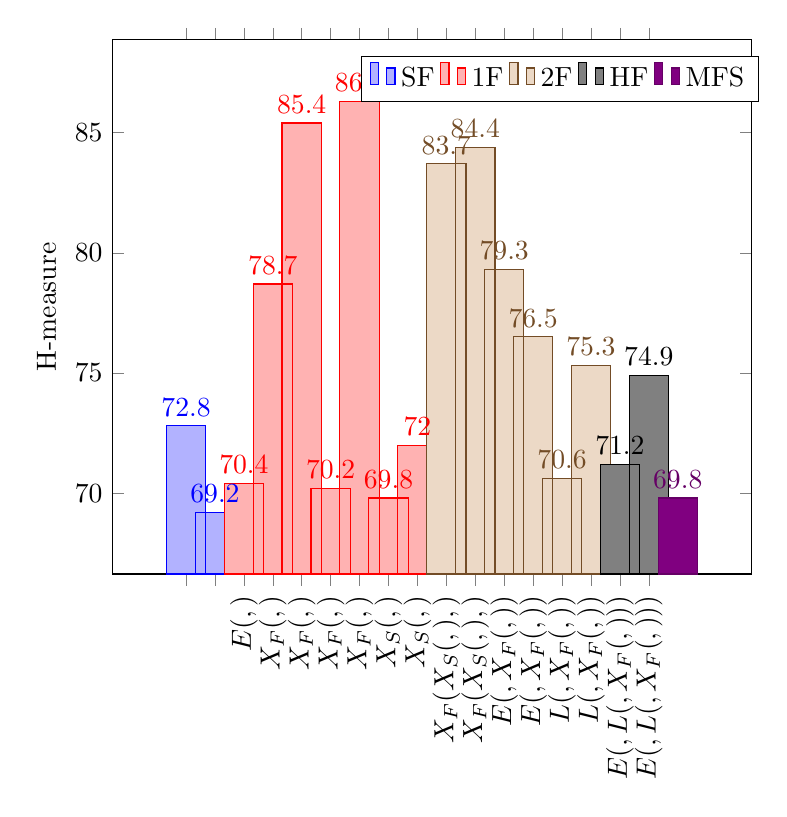
\begin{tikzpicture}{width=15cm,height=5cm}
\pgfplotsset{compat=1.8}
\begin{axis}[
%	xtick distance={160},
    ybar=-0.5cm,
    width=.8\linewidth,
    enlargelimits=0.15,
    domain = 0:85,
    xmin=0, xmax=85,
%    x=1mm, % Distance between the centers of the bars
%    enlarge x limits={abs=1cm}, % The distance between the center of the first bar and the left edge
%    enlarge y limits=false,
    legend style={at={(0.7,.97)},anchor=north,legend columns=-1},
    ylabel={H-measure},
%    xmin=0, xmax=85,
    xticklabels={
	    {$\mlex$},
	    {$\msyn$},
	    {$E(\mlex, \msyn)$},
	    {$X_F(\slex, \mlex)$},
	    {$X_F(\slex, \msyn)$},
	    {$X_F(\ssyn, \mlex)$},
	    {$X_F(\ssyn, \msyn)$},
	    {$X_S(\ssyn, \slex)$},
	    {$X_S(\slex, \ssyn)$},
	    {$X_F(X_S(\slex, \ssyn), \mlex)$},
	    {$X_F(X_S(\slex, \ssyn), \msyn)$},
	    {$E(\mlex, X_F(\slex, \mlex))$},
	    {$E(\msyn, X_F(\slex, \mlex))$},
	    {$L(\msyn, X_F(\slex, \msyn))$},
	    {$L(\mlex, X_F(\slex, \mlex))$},
	    {$E(\mlex, L(\msyn, X_F(\slex, \msyn)))$},
	    {$E(\mlex, L(\mlex, X_F(\slex, \mlex)))$}
    },
    xtick={0,5,...,80},
    nodes near coords,
    nodes near coords align={vertical},
    x tick label style={rotate=90,anchor=east},
    ]
\addplot+[mark=none, bar width=.5cm]  coordinates {(0,72.8) (5,69.2)};
\addplot+[mark=none, bar width=.5cm]  coordinates {(10,70.4) (15,78.7) (20,85.4) (25,70.2) (30,86.3) (35,69.8) (40,72.0)};
\addplot+[mark=none, bar width=.5cm]  coordinates {(45,83.7) (50,84.4) (55,79.3) (60,76.5) (65,70.6) (70,75.3)};
\addplot+[mark=none, bar width=.5cm]  coordinates {(75,71.2) (80,74.9)};
\addplot+[mark=none, bar width=.5cm]  coordinates {(85,69.8)};

\legend{SF,1F,2F,HF, MFS}
\end{axis}
\end{tikzpicture}
\caption{H-measure for the WSI/WSD task on the Semeval 2007 corpus. Results are obtained with the spectral clustering algorithm.}
% The best performing operator is the $X_F(\slex,\mlex)$.}
\label{fig:h_measure_semeval2007}
\end{figure}


In the following subsection, we put aside the fusion enrichment and we focus into another characteristic of our proposed hypergraph structure. We leverage the links (features) among nodes (words) to induce senses. Specifically, we propose a method that clusters together words which represent induced senses for a set of target words.


\subsection{Leveraging the Linguistic Network Structure}
Until now, we have employed the hypergraph representation in terms of leveraging the heterogeneous information to enrich and densify a feature space.
Now, we will leverage the relations that exist within the network to identify words that, together with their neighborhood, represent a sense. Thus, we propose a network-based algorithm to solve word sense induction. 

%Word sense disambiguation, or WSD, is the task of examining a word in different contexts (we refer to a word in a particular context as an instance)  and determining which is the sense being used in each one of the contexts analyzed. Usually a list of senses from where to chose the correct one is given as an input. When this list is not available, WSD then becomes a different, complementary task: word sense induction, or WSI. WSI also analyzes  tokens of a target word context but before assigning a sense to each of its instances, it first generates a list of possible senses from where to select from. 





%

%\paragraph{State of the art discussion}\label{sec:survey_disc}


With respect to the information contained in the network, we find that few approaches include syntactic attributes into their model. We believe that finding semantic similarities can be improved by leveraging syntactic information by using dependency relations. 
%Moreover, using syntactic data along with semantic and/or lexical co-occurrences takes us into the heterogeneous network domain which has not been addressed in most of the approaches covered.
%Being able to design new similarity metrics that deal with different types of information opens new avenues of research in the semantic similarity domain. % Finally, concerning the algorithms employed, few approaches make direct use of the graph Laplacian representation. New similarities could be defined using the Laplacian as a starting point. 




\paragraph{Proposed Method}
	
%The cited works use a LCN as described before while other works such as \cite{2014.Tao.Qian.LexicalChainHypergraphWSI} represent the co-occurrence by means of a hypergraph schema. In short, a hypergraph structure is a graph generalization where an edge (called hyperedge) can link multiple vertices per edge and thus it is able to provide a more complete description of the interactions between several nodes.


Formally, the objective of WSI/WSD is the following: given a document $d$ with a set $T$ of  target words $tw \in T$ and the set $C$ with contexts for each target word $ct_{tw}$. 
Specifically, each paragraph represents the context  of a target word. A target word in a specific context is also called an instance.
% $tw$. %Each word $tw$ features several $ct$.
The goal is first to solve the WSI task, that is, automatically determine a list of senses for a given $tw$, and then assign one meaning from this list to each of its instances, the WSD task.
%
%As described before, WSI  is usually solved following four steps: (1) creation of a linguistic network, (2) determine the level of similarity between nodes within the network, (3) cluster nodes together, thus creating individual senses, and (4)  assign a cluster (sense) to each instance of a target word in the input document (this step amounts to WSD).


Our method  is inspired on previous approaches from both \cite{2004.Veronis} and \cite{2007.Klapaftis.UOY}. In Hyperlex,  the graph-based  method presented  in \cite{2004.Veronis}, the main intuition is that co-occurrence networks have small-world properties and thus it is possible to detect and isolate important heavily-connected nodes, called "hubs". These hubs, and their connected nodes represent a sense in itself. 

Hyperlex performs WSI and WSD using a weighted lexical co-occurrence network. The process is performed for each target word in the document. As a first step, they build a  graph by defining the vertices (the target word node is removed) as the tokens found in the  co-occurring  context of a target word. The edges link two words co-occurring together. Each edge is assigned a weight that decreases as the association frequency of the words increases. The second step consists on iteratively finding the hubs and removing them, along with their adjacent nodes, from the target word graph. Again, the intuition of the method is that these isolated hubs, and their adjacent words, represent a sense of the analyzed word. The third and final step carries out the disambiguation. A new graph is created by adding the target word to the co-occurrence graph. Zero-weighted edges are added between each hub and the target word. A minimum spanning tree is then calculated and the sense component found to have the closest set of nodes is chosen as the target word sense.

The second approach, {UoY}, described in \cite{2007.Klapaftis.UoY},  relies itself on the small-world intuition presented  by Hyperlex to find hubs and its adjacent nodes to represent senses.   In short, these methods, as ours, exploit the real-world characteristics of linguistic networks by theorizing that there are certain few high-degree nodes (called hubs) that carry an important role in the network and therefore may represent, coupled with their neighbors, a sense for a given target word. Particularly, UoY considers bigrams and trigrams that co-occur in a paragraph as hyperedges. Under a frequent-itemset setting, they determine important hyperedges given their \textit{support} and their \textit{confidence}  values. Then, the clustering of words takes place by finding the hubs and considering them as sense carriers only if they satisfy a threshold mainly set upon their containing-hyperedge confidence value. Finally, once the senses are identified, each target word instance (represented by a context) is assigned to a sense according to the sum of confidences of the hyperedge appearing on said context. 

In our method, we generate a network for each $tw$ and consider that the high-degree nodes inside this network may represent a $tw$ sense. Figure \ref{fig:wsd_wsi_process}  shows an overview of the process. Also, in Algorithm \ref{alg:wsd} we show the general flow of our approach.  We detail the steps taken alongside the corresponding line in the algorithm below. 

\begin{figure}
\centering
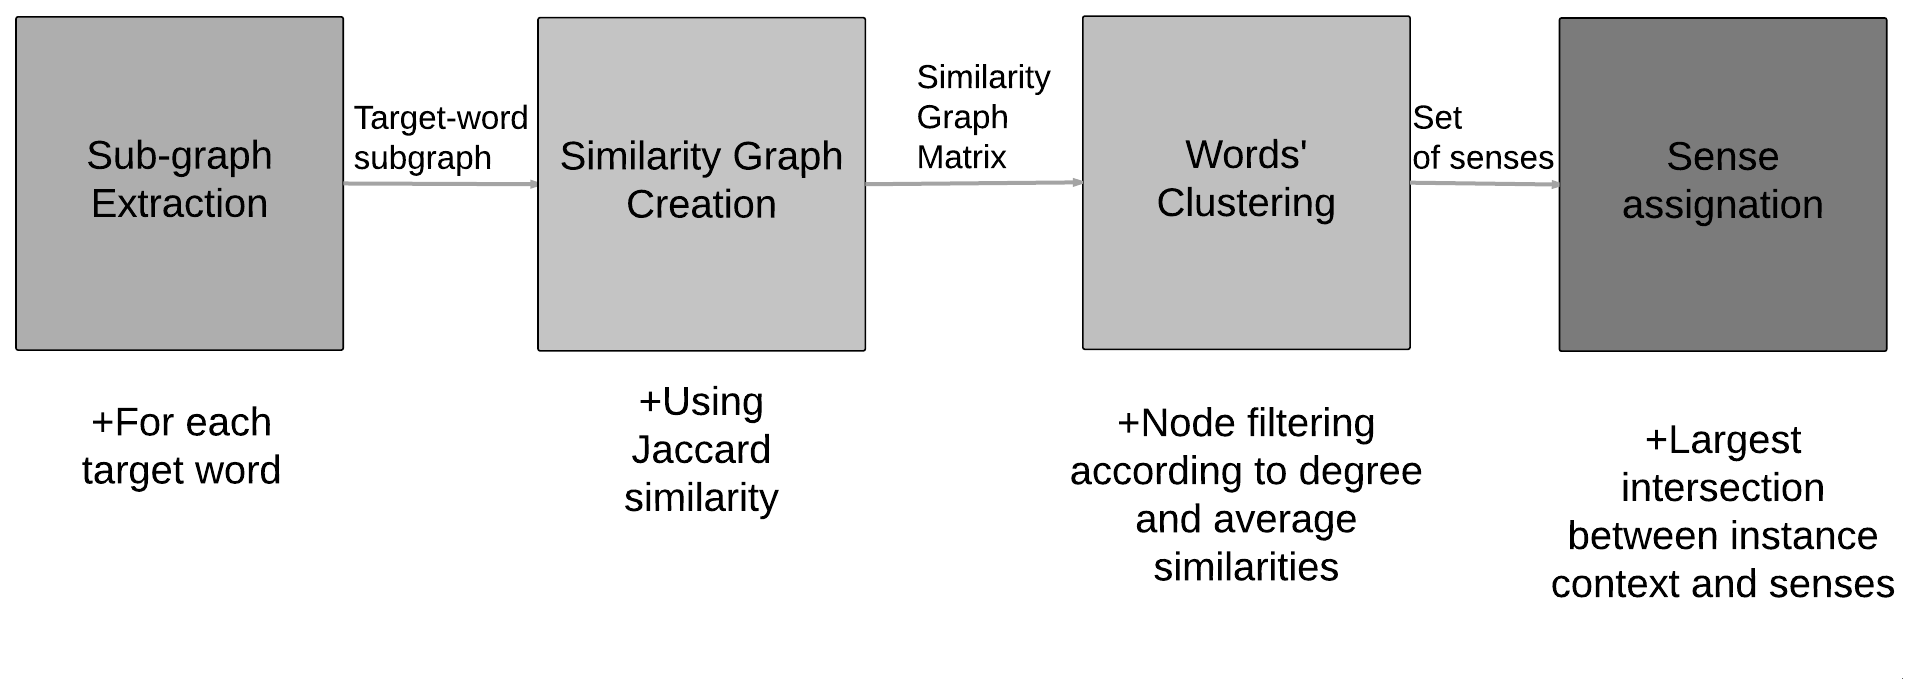
\includegraphics[width=1\linewidth]{images/Chapitre4/wsd_wsi_process.png}
\caption{Block diagram of the WSI/WSD method proposed.}
\label{fig:wsd_wsi_process}
\end{figure}


\paragraph{Creation of the linguistic network}
%In the previous sections we worked with the English Wikipedia as background corpus to build and model our proposed linguistic network. Given the large size of Wikipedia, and to iterate faster our experiments, we decided to change the corpus to one with a more manageable size.

%We use the Open American National Corpus (OANC) \cite{oanc} as background document collection to build a hypergraph network $G_H$ following our proposed model.  The OANC  includes texts from several domains and encompasses 11,406,155 words. We split the documents of the corpus in sentences, then we tokenize and parse them with Stanford's CoreNLP \cite{corenlp}. As described before, the dependency and constituency tree are used to build the hypergraph: words are depicted by nodes, and they may exist inside any of the three different types of hyperedges defined (sentence,  noun phrase or dependency contexts). If any  hyperedge is repeated through the corpus, we increment a counter and keep the number of apparitions instead of adding redundant columns to the hypergraph incidence matrix.

\begin{algorithm}[!htp]
\SetAlgoLined
\KwIn{A set $tw\_set=\{tw_1, tw_2, ..., tw_n\}$ of target words }
\KwIn{A background linguistic network $G_H$}
\KwIn{Filtering thresholds $th_1$, $th_2$}

\KwOut{A set $SoS_{tw}$ of senses for each target word}
\ForEach{target word $tw$ in tw\_set}{
	
	$G_{tw}$ = \texttt{extract\_subgraph}($G_H$, $tw$)\;
	$B_{tw}$ = \texttt{induce\_bipartite\_graph}($G_{tw}$)\;
	$S_{tw}$ = \texttt{sim\_matrix}($B_{tw}$)\;
	$F_{tw}$ = \texttt{induce\_hypergraph}($S_{tw}$, \textit{th1})\;
	$candidate\_hubs$ = \texttt{sort(degree}($F_{tw}$))[:100]\;
	$SoS_{tw}$ = [~]\;
	\ForEach{candidate\_hub in candidate\_hubs}{
%		\uIf{\texttt{degree}(candidate\_hub) $<$ th2}{
%			\textbf{continue}\;
%			}
%		\tcc{get all hyperedges where candidate\_hub appears}
		$candidate\_hyperedges$ = \texttt{get\_hyperedges}($candidate\_hub$, $F_{tw}$)\;
		$candidate\_avg_jaccard$ = 0\;
		\ForEach{ hyperedge in candidate\_hyperedges}{
%		\tcc{get average jaccard of all words (nodes) within hyperedge}
			$candidate\_avg\_jaccard$ += \texttt{get\_avg\_jaccard}($hyperedge$)\;
			}
		\uIf{candidate\_jaccard $>$ th2}{
			$SoS_{tw}$.\texttt{add}(\texttt{get\_words}($candidate\_hyperedges$))\;
%			\tcc{remove hyperedges of candidate hub from tw (filtered) hypergraph.}
			$F_{tw}$ = $F_{tw} \setminus candidate\_hyperedges$\;
		}
	}
	\Return{$SoS_{tw}$}
}

\caption{Pseudo-code of our WSI/WSD network-based approach}
\label{alg:wsd}
\end{algorithm}


In order to find senses from the contexts of a target word, the first step in our procedure is to build a linguistic graph $G_H$ from a background corpus. As described in previous sections, the dependency and constituency trees are used to build the hypergraph: words are depicted by nodes, and they may exist inside any of the three different types of hyperedges defined (sentence,  noun phrase or dependency contexts). If any  hyperedge is repeated through the corpus, we increment a counter and keep the number of apparitions instead of adding redundant columns to the hypergraph incidence matrix.

At each step, that is, for each $tw$ in the test input document, we extract a subgraph $G_{tw}$ from $G_H$ that contains all the words that appear together with $tw$ (line 2), whether by lexical or syntactic co-occurrence. The $tw$ is removed from $G_{tw}$. In this approach we focus specifically on dependency relations and lexical co-occurrence. 

We note that for the syntactic co-occurrence, that is, the dependency relations between words, we apply two strategies: when dealing with a noun target word, we use the co-occurrent relations between said noun and other words having a similar  dependency head token. On the other hand, when dealing with a verb target word, we select the co-occurrent words having said verb as head of the dependency relation.  The reason is that usually verbs are more often than not the head of dependency relations, so the intuition is that words which have the same verb governor are somehow semantically related. %Otherwise, if we took the relations between verbs and other words having a similar dependency head, we would 

\paragraph{Computing the similarity between nodes}
In order to computationally treat $G_{tw}$, we first induce a bipartite graph $B_{tw}=(U,W,E)$ from $G_{tw}$ (line 3). The set of left nodes $U$ represent words and the set of right nodes $W$ depicts the membership to a given hyperedge. Thus, we have as many nodes in $W$  as we had hyperedges in $G_H$.

We compute the Jaccard index between each node $n_{i,j} \in U$ as $Jaccard(i,j)=\frac{|N(i)\cap N(j)|}{|N(i)\cup N(j)|}$ in order to build a $|U|\times|U|$ similarity matrix $S_{tw}$ (line 4). We induce from $S_{tw}$ a new filtered  hypergraph incidence matrix $F_{tw}$ (line 5), which contains word nodes as rows and columns as hyperedges. Each of these hyperedges represent a set of words that are deemed similar between them according to their Jaccard  index value, which must be equal or higher than an assigned threshold $th_1$ .  

\paragraph{Clustering words  together}
Once the incidence matrix $F_{tw}$ is built we can proceed to induce senses for a target word by clustering words (vertices) together. First, we calculate the degree of each node $n_i \in F_{tw}$. The degree of a node is simply the number of hyperedges it is incident in. Nodes are sorted in descending order and evaluated one by one. We consider the top $c$-nodes as sense hub candidates (line 6). We accept or reject a node $n \in F_{tw}$ as a sense carrying word according to one condition. As shown from line 11 to 17 in the pseudo-code, we set a minimum limit to the average of the Jaccard similarities between each pair of neighbors of node $n \in F_{tw}$ within each hyperedge  $n$ belongs to. Formally, for a node $n$, we define the average Jaccard measure as: $$AvgJaccard(n)=\frac{1}{|hedges(n)|}\sum_{h\in hedges(n)}\frac{\sum_{\substack{i\in h\\j\in h;i\neq j}}Jaccard(i,j)}{|h|}$$ 
where $hedeges(n)$ is the set of hyperedges $n$ is incident in and its cardinality is defined as $|hedges(n)|$, and $|h|$ is the number of nodes in the hyperedge $h$. 

The Jaccard similarity measure allows us to easily determine the neighbors of each node in the current bipartite hypergraph representation. As each node is joined to a sentence or dependency node, calculating the Jaccard similarity amounts to determining the level of co-occurrence between each word according to a specific type of hyperedge (represented as a node from the other graph partition) while taking into account the total number of hyperedges the words participate in. We differentiate specifically from the previously described method, UoY, in that in the case of that system, the weighting of the hyperedges is done by computing the average confidence metric of each hyperedge. In this regard, the Jaccard similarity is more flexible with respect to the confidence metric, as the confidence requires in the numerator the number of contexts (paragraphs in UoY's case) shared by all the members of the hyperedge, whereas the Jaccard measure takes pairs of members individually and thus is less strict in the apparition of all the elements of the hyperedge in the contexts. Given the nature of the features used (lexical and syntactical dependencies), we fix our thresholds in a manual but simpler way by defining percentiles and taking the value of the threshold directly, without having to change it according to the characteristics of the data.

If node $n$ satisfies both thresholds $th_1$ and $th_2$, it is deemed as a sense purveyor and all its neighbors (words that appear in the same hyperedges as $n$) are conflated into a single set representing a $tw$ sense. This new sense is added to $SoS_{tw}$ (line 17). The sense set is then removed from $F_{tw}$.

The process is repeated until no more nodes satisfy both boundaries. When the process is complete, we obtain a set of senses $SoS_{tw}$ where each set contains words that ideally represent a unique meaning for each target word. 

\paragraph{Sense assignation}

The assignation of a sense consists in looking at each $tw$ instance represented by a context $ct$ and simply determining which sense $s$ in $SoS_{tw}$ shares the highest amount of words with $ct$. The sense $s$ is thus assigned to that instance. If two senses in $SoS_{tw}$ share the same amount of words with $ct$, one of them is randomly chosen.  This operation is repeated for each instance of each target word. 



	
\subsection{Experiments and Evaluation}
\paragraph{Test Datasets}
We trained and evaluated our system on two datasets: Semeval 2007 Task 2 (as in the previous experiments) and Semeval 2010 Task 14 \cite{Semeval2010}. We recall that the Semeval 2007 task consisted in the induction and disambiguation of a single set of 100 words, 65 verbs and 35 nouns, each target word having a set of contexts where the word appear. The average number of senses in the testing set is 2.87. On the other hand, the Semeval 2010 task consisted also on 100 words, with 50 being verbs and 50 being nouns. The average number of true senses in this dataset is 3.79. On this version of Semeval, a training set from which the senses of a word have to be induced is provided. In our experiment, for the Semeval 2010 dataset, we induce the senses from the training set and disambiguate the target words present within the test set.

We apply a light pretreatment, consisting on token lemmatization and we remove all words that appear less than four times. Concerning the individual graphs of each target word, we work only with nouns and if the extracted graph has fewer than 100 nodes, we do not apply any filtering (we keep all the extracted words). We do this in order to avoid empty solutions.



\paragraph{Implementation}
The objective of this experiment is to understand the performance of both lexical and syntactic co-occurrence information, used independently, while solving WSI and WSD tasks while using the method described in the previous subsection. To that end we build two independent systems, using : $\mlex$, which uses exclusively lexical co-occurrence hyperedges, and $\msyn$, which employs only syntactic dependency hyperedges. Both are obtained as described in Chapter \ref{chap:ling_net}, section \ref{sec:ling_model}.
 %
 
Each type of hyperedge has its own network characteristics as mentioned before. Sentence hyperedges tend to have a much smaller number of words than those of the dependency category. This make sense as sentences usually contain less than 30 words, meanwhile a dependency hyperedge may contain up to hundreds of words (several words may share the same dependency relation). Taking this into consideration we set different threshold values for $\mlex$ and for $\msyn$. First, we  consider only the top 100 nodes as candidate sense hubs. Secondly, we do not set the thresholds' values directly but instead we experimentally set up a percentile value for the Jaccard similarity ($th_1=30$) and for the average Jaccard similarity ($th_2=30$). This is a practical solution to the changing nature of the network model according to the features being employed. We experimentally found the best values for  each threshold used.



%Given that the variation of these thresholds affect the performance of the systems, we decided to experimentally fix threshold $th_1$ at 0.7 for \textit{dep} and at 0.030 for \textit{lex}. The difference of scales is determined by the characteristics stated before, that is, the sparse nature of the sentence hyperedges compared to the density of dependency hyperedges. The second threshold $th_2$ is automatically set for both systems, as explained above.
%
%This leaves only one threshold left, $th_3$. We experiment with two different ranges of values, one for each system. For \textit{dep} we set the range $[0.3, 0.65]$ with a step of 0.05. For \textit{lex} we set $[0.01, 0.08]$ with a step of 0.1. These ranges were chosen experimentally with two constraints in mind: (1) lower threshold values usually gave the same results\footnote{Still, some of the values used produced equal results and thus are not visible in Figure \ref{fig:prec_recall}.} as those already included in our ranges, and (2) higher threshold values forced the system to either give only one sense per word (resulting in the most frequent baseline), or even worse, not accepting any sense, thus having an null solution. 



\paragraph{Results and Discussion}
Both Semeval 2007 and Semeval 2010 tasks are first evaluated by an unsupervised and supervised set of measures, as before. Later on, we present the results according to our H-measure. The objective of these results comparison is to determine the level of performance of our proposed method and to verify that the fusion-produced representation spaces do improve over the use of independent features and the trivial feature concatenation (with early fusion).

\subparagraph{Semeval 2007}



\begin{table}[htp!]
\centering
%\setlength\tabcolsep{3pt}
\caption{All-words, nouns, and verbs supervised recall for the Semeval 2007 corpus using fusion operations (SF, 1F, 2F, HF) and our proposed method. We also display the average number of clusters found by each fusion configuration, the best performing system as well as the MFS baseline. In bold the best results per-column among our experiments.}
\label{tab:sem2007_PM_Recall}
\begin{tabular}{@{}lrrrrc@{}}
\toprule
\textbf{Fusion Operation / System} & \multicolumn{3}{c}{\textbf{Recall (\%)}} & \#\textbf{cl} & \textbf{Fusion Level}\\ 
        & \textbf{all}          & \textbf{nouns}          & \textbf{verbs} &          \\ 
       \midrule
        \multicolumn{5}{r}{\textbf{Single Features}} & \multirow{3}{*}{\textbf{SF}} \\ %\midrule
       $\mlex$                    & 78.70 & 81.00 & 76.00 & 4.21\\
 

       $\msyn$                    & 78.41 & 80.30 & 76.10 & 2.26\\
       \midrule
                   \multicolumn{5}{r}{\textbf{Early Fusion (EF)}}  & \multirow{10}{*}{\textbf{1F}}     \\ %\midrule
       $E(\mlex, \msyn)$		& 78.80 & 81.00 & \textbf{76.40} & 2.43\\
	  %\midrule
                   \multicolumn{5}{r}{\textbf{Cross Feature Fusion ($\mathbf{X_FF}$)}}       \\ %\midrule	         
	   
	   $X_F(\slex, \mlex)$		& 78.70 & 80.90 & 76.20  & 3.11\\	   
       $X_F(\slex, \msyn)$		& 78.50 & 81.10 & 75.60  & 1.92\\
	   $X_F(\ssyn, \mlex)$		& \textbf{79.10} & \textbf{81.60} & \textbf{76.40}  & 1.73\\	   
       $X_F(\ssyn, \msyn)$		& 78.60 		 & 80.90  & 76.00 & 1.81\\       
 %\midrule
                   \multicolumn{5}{r}{\textbf{Cross Similarity Fusion ($\mathbf{X_SF}$)}}       \\ %\midrule
	   
 
	   $X_S(\ssyn, \slex)$		& 78.60 & 80.80 & 76.20  & 1.44\\
	   $X_S(\slex, \ssyn)$		& 78.70 & 80.90	& 76.20 & 1.10\\
	  
 \midrule
                   \multicolumn{5}{r}{\textbf{Cross Feature Cross Similarity Fusion ($\mathbf{X_FX_SF}$)}}  & \multirow{9}{*}{\textbf{2F}}     \\ %\midrule
	   
       $X_F(X_S(\slex, \ssyn), \mlex)$		& 78.70 & 81.00 & 75.80 & 1.59 \\	   
       $X_F(X_S(\slex, \ssyn), \msyn)$		& 78.70 & 81.00 & 76.10 & 1.38\\	   
       	  %\midrule
                   \multicolumn{5}{r}{\textbf{Early Cross Feature Fusion ($\mathbf{EX_FF}$)}}       \\ %\midrule	         
       
       $E(\mlex, X_F(\slex, \mlex))$		&78.70 & 81.20 & 75.80 & 2.41\\	   
	   $E(\msyn, X_F(\slex, \mlex))$		& 78.90 & 81.40 & 76.10 & 2.35\\	   
       %\midrule
                   \multicolumn{5}{r}{\textbf{Late Cross Feature Fusion ($\mathbf{LX_FF}$)}}       \\ %\midrule	  
	   $L(\msyn, X_F(\slex, \msyn))$		& 78.50 & 81.10 & 75.60 & 1.91\\	   
	   $L(\mlex, X_F(\slex, \mlex))$		& 78.70 & 80.80 & \textbf{76.40} & 3.12\\	   
       \midrule
                   \multicolumn{5}{r}{\textbf{Early Late Cross Feature Fusion ($\mathbf{ELX_FF}$)}}     & \multirow{3}{*}{\textbf{HF}}  \\ %\midrule	  
	   $E(\mlex, L(\msyn, X_F(\slex, \msyn)))$		& 78.60 & 80.70 & 76.20 & 1.99\\	   
	   $E(\mlex, L(\mlex, X_F(\slex, \mlex)))$		& 78.60 & 81.10 & 75.70 & 2.39\\
	   \midrule
	   \midrule
	   

	   Baseline MFS		& 78.70 & 80.90 & 76.20 & 1.00\\ 	   	 	    
%	   Semeval 2007 Best System& 81.60 & 86.80 & 75.70 & 1.15\\ 	 		   
       \bottomrule
\end{tabular}
\end{table}


\begin{table}[htp!]
\centering
\setlength\tabcolsep{3pt}
\caption{All-words, nouns, and verbs unsupervised F-measure for the Semeval 2007 corpus using fusion operations (SF, 1F, 2F, HF) and our proposed method. We also display the average number of clusters found by each fusion configuration, the best performing system as well as the MFS baseline. In bold the best results per-column among our experiments.}
\label{tab:sem2007_PM_unsup_FS}
\begin{tabular}{@{}lrrrrc@{}}
\toprule
\textbf{Fusion Operation / System} & \multicolumn{3}{c}{\textbf{F-measure (\%)}} & \#\textbf{cl} & \textbf{Fusion Level}\\ \midrule
      	& \textbf{all}          & \textbf{nouns}          & \textbf{verbs}           \\ 
       \midrule
       \multicolumn{5}{r}{\textbf{Single Features}} & \multirow{3}{*}{\textbf{SF}}\\ %\midrule
       $\mlex$                    &	63.80	 & 61.30 & 66.50 & 4.21\\
 

       $\msyn$                    &	75.90	& 78.80 & 72.60 & 2.26\\
       \midrule
       \multicolumn{5}{r}{\textbf{Early Fusion (EF)}}  & \multirow{10}{*}{\textbf{1F}}     \\ %\midrule
       $E(\mlex, \msyn)$		&	76.90	& \textbf{80.20} & 73.10 & 2.43\\
	  %\midrule
       \multicolumn{5}{r}{\textbf{Cross Feature Fusion ($\mathbf{X_FF}$)}}       \\ %\midrule	         
	   
	   $X_F(\slex, \mlex)$		&	71.00	& 68.10 & 74.20 & 3.11 \\	   
       $X_F(\slex, \msyn)$		&	77.70	& 79.60 & 75.50 & 1.92 \\
	   $X_F(\ssyn, \mlex)$		&	75.20	& 75.50 & 74.90	 & 1.73 \\	   
       $X_F(\ssyn, \msyn)$		&	77.60	& 80.50 & 74.30 & 1.81 \\       
% \midrule
       \multicolumn{5}{r}{\textbf{Cross Similarity Fusion ($\mathbf{X_SF}$)}}       \\ %\midrule
	   
 
	   $X_S(\ssyn, \slex)$		&	74.10	& 72.10 & 76.50 & 1.44 \\
	   $X_S(\slex, \ssyn)$		&	\textbf{78.30}	& 79.70  & \textbf{76.80} & 1.10 \\
	  
 \midrule
       \multicolumn{5}{r}{\textbf{Cross Feature Cross Similarity Fusion ($\mathbf{X_FX_SF}$)}}   & \multirow{9}{*}{\textbf{2F}}    \\ %\midrule

       $X_F(X_S(\slex, \ssyn), \mlex)$		&	77.80	&79.10  & 76.40& 1.59 \\	   
       $X_F(X_S(\slex, \ssyn), \msyn)$		&	75.90	& 75.60 & 76.30 & 1.38 \\	   
       	  %\midrule
       \multicolumn{5}{r}{\textbf{Early Cross Feature Fusion ($\mathbf{EX_FF}$)}}       \\ %\midrule	         
       
       $E(\mlex, X_F(\slex, \mlex))$		&	75.40	& 76.30  & 74.40 & 2.41 \\	   
	   $E(\msyn, X_F(\slex, \mlex))$		&	73.80	& 72.80  & 74.80 & 2.35 \\	   
       %\midrule
       \multicolumn{5}{r}{\textbf{Late Cross Feature Fusion ($\mathbf{LX_FF}$)}}       \\ %\midrule	  
	   $L(\msyn, X_F(\slex, \msyn))$		&	77.60	& 79.50	 & 75.50 & 1.91 \\	   
	   $L(\mlex, X_F(\slex, \mlex))$		&	70.10	& 67.70 & 74.20 & 3.12 \\	   
       \midrule
       \multicolumn{5}{r}{\textbf{Early Late Cross Feature Fusion ($\mathbf{ELX_FF	}$)}}    & \multirow{3}{*}{\textbf{HF}}   \\ %\midrule	  
	   $E(\mlex, L(\msyn, X_F(\slex, \msyn)))$		&	77.90	& 79.50 & 75.80& 1.99 \\	   
	   $E(\mlex, L(\mlex, X_F(\slex, \mlex)))$		&	75.40	& 76.30&74.40 & 2.39 \\
	   \midrule
	   \midrule
	   Baseline 1c1word 		&	78.90	& 80.70&76.80 & 1.00 \\ 	   	 	    	   
%	   Semeval 2007 Best Systems	&	78.70	& 80.80&76.30 & 3.06 \\ 	 

		   
       \bottomrule
\end{tabular}
\end{table}


In Table \ref{tab:sem2007_unsup_FS} we present the unsupervised F-measure evaluation results for our models as well as for some other systems: the previously presented UoY (version 2007) and UBC-AS \cite{Agirre2007UBC}, the best performing system according to this measure. Additionally, three baselines are included, the already-known 1c1word plus two new ones, the Random  baseline which assigns a sense randomly to each test instance; and the 1c1instance baseline, which attributes a unique sense to each one of the test instances. Finally, we also include the fusion operator that obtained the highest performance (according to the H-measure) in the experiments of the previous subsection, that is, the results of the $X_F(\slex,\mlex)$ fusion. As the last experiments were performed with spectral clustering, we will call this system SC$_\text{fusion}$. Furthermore, given that we generate representation spaces, we can use the same fusion matrix but this time using the graph-based algorithm presented in this subsection, instead of the spectral clustering used before. We call this system GB$_{\text{fusion}}$

In this table, as in the rest of the tables presented in this section, as before, the columns show the results for all the words, for the nouns, and for the verbs. Again, the final column indicates the number of induced clusters per system. It is important to consider this value as the unsupervised metrics are biased towards systems with less number of induced clusters and thus to the 1c1word baseline. We aim to address this shortcoming with our H-measure.

Looking at the table, we can see that both our methods surpass the baselines and the system described before {UoY(2007)}. The best system of the competition, {UBC-AS} used also co-occurrence graphs and applied a random-walk based clustering algorithm over the vertices' similarity matrix. Still, our system induced a larger amount of senses, while retaining a competitive F-measure value. We also note that in this evaluation $\msyn$, the system using only co-occurrent dependency relations outperformed the lexical co-occurrence only system $\mlex$. It is very possible that this lack of lexical performance is due to the size of the surrounding words window, which in this case is selected to be the entire phrase were the word occurs. 

With respect to our fusion space methods, SC$_{\text{fusion}}$ and GB$_{\text{fusion}}$ we find that both are competitive but cannot achieve a better performance that those systems prepared for the competition. Both systems are better than using independent features, according to the unsupervised F-measure. GB$_{\text{fusion}}$  Nonetheless, for supervised recall, only GB$_{\text{fusion}}$ beats both of the single feature matrices.

\begin{figure}
\centering
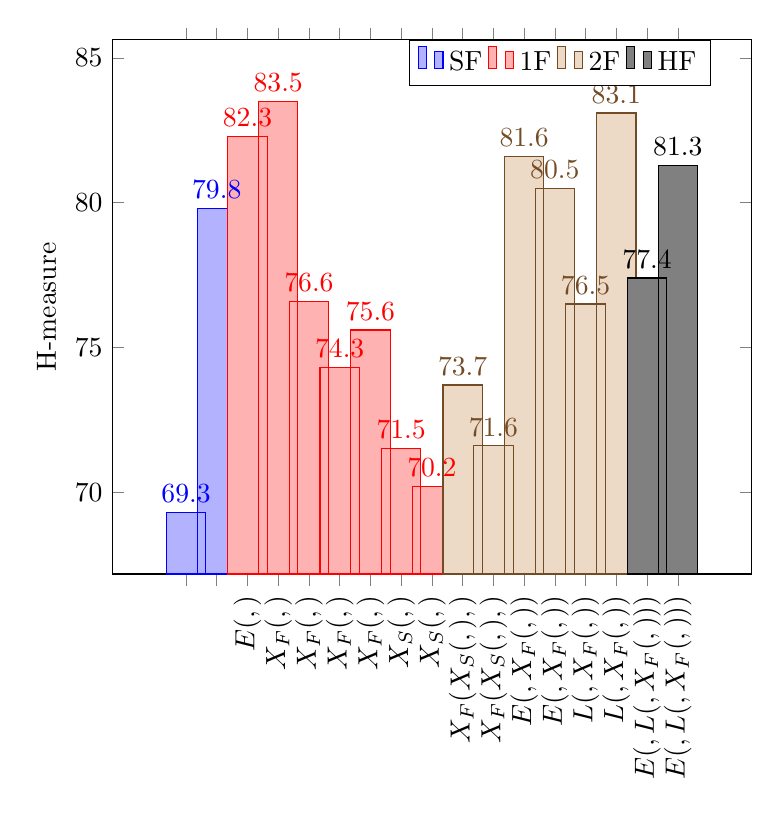
\begin{tikzpicture}{width=15cm,height=5cm}
\pgfplotsset{compat=1.8}
\begin{axis}[
%	xtick distance={160},
    ybar=-0.5cm,
    width=.8\linewidth,
    enlargelimits=0.15,
    domain = 0:80,
    xmin=0, xmax=80,
%    x=1mm, % Distance between the centers of the bars
%    enlarge x limits={abs=1cm}, % The distance between the center of the first bar and the left edge
%    enlarge y limits=false,
    legend style={at={(0.7,1)},anchor=north,legend columns=-1},
    ylabel={H-measure},
%    xmin=0, xmax=85,
    xticklabels={
	    {$\mlex$},
	    {$\msyn$},
	    {$E(\mlex, \msyn)$},
	    {$X_F(\slex, \mlex)$},
	    {$X_F(\slex, \msyn)$},
	    {$X_F(\ssyn, \mlex)$},
	    {$X_F(\ssyn, \msyn)$},
	    {$X_S(\ssyn, \slex)$},
	    {$X_S(\slex, \ssyn)$},
	    {$X_F(X_S(\slex, \ssyn), \mlex)$},
	    {$X_F(X_S(\slex, \ssyn), \msyn)$},
	    {$E(\mlex, X_F(\slex, \mlex))$},
	    {$E(\msyn, X_F(\slex, \mlex))$},
	    {$L(\msyn, X_F(\slex, \msyn))$},
	    {$L(\mlex, X_F(\slex, \mlex))$},
	    {$E(\mlex, L(\msyn, X_F(\slex, \msyn)))$},
	    {$E(\mlex, L(\mlex, X_F(\slex, \mlex)))$}
    },
    xtick={0,5,...,80},
    nodes near coords,
    nodes near coords align={vertical},
    x tick label style={rotate=90,anchor=east},
    ]
\addplot+[mark=none, bar width=.5cm]  coordinates {(0,69.3) (5,79.8)};
\addplot+[mark=none, bar width=.5cm]  coordinates {(10,82.3) (15,83.5) (20,76.6) (25,74.3) (30,75.6) (35,71.5) (40,70.2)};
\addplot+[mark=none, bar width=.5cm]  coordinates {(45,73.7) (50,71.6) (55,81.6) (60,80.5) (65,76.5) (70,83.1)};
\addplot+[mark=none, bar width=.5cm]  coordinates {(75,77.4) (80,81.3)};
%\addplot+[mark=none, bar width=.5cm]  coordinates {(85,69.8)};

\legend{SF,1F,2F,HF, MFS}
\end{axis}
\end{tikzpicture}
\caption{H-measure for the WSI/WSD task on the Semeval 2007 corpus. Results are obtained with our proposed  algorithm.}
\label{fig:h_measure_PM_semeval2007}
\end{figure}

\begin{table}[!tb]
\centering
\caption{Supervised Recall (SR) on the Semeval 2007 test set. The highest values for each column are in bold. Results are obtained with our proposed algorithm.}
\begin{tabular}{@{}lrrrr@{}}
\toprule
\textbf{System} & \multicolumn{3}{c}{\textbf{Recall (\%)}} & \textbf{\#cl} \\
 & \textbf{all} & \textbf{nouns} & \textbf{verbs} & \\ \midrule
I2R & \textbf{81.6} & \textbf{86.8} & 75.7 & 3.1 \\
GB$_{\text{fusion}}$ & 79.6 & 83.3 & {76.3} & 3.4 \\
$\mlex$ & 79.4 & 82.5 & 75.9 & 4.3 \\
SC$_{\text{fusion}}$ & 79.2 & 82.3 & 75.7 & 3.6\\
$\msyn$ & 79.1 & 81.5 & \textbf{76.4} & 3.3\\
MFS & 78.7 & 80.9 & 76.2 & 1.0 \\
UoY(2007) & 77.7 & 81.6 & 73.3 & 9.3 \\ \bottomrule
\end{tabular}

\label{tab:sem2007_sup_recall}
\end{table}

Moving onto the supervised results for Semeval 2007, in Table \ref{tab:sem2007_sup_recall} we show the results obtained concerning supervised recall.  In this table we include the competing system I2R \cite{Niu2007}, based on an Information Bottleneck based clustering algorithm, which obtains the best results according to all the words and nouns. Both our systems $\msyn$ and $\mlex$ beat the baseline of assigning the most frequent sense to an instance MFS). More interestingly, $\msyn$ was able to beat the MFS verb baseline, something that was not achieved during the competition. As was the case before, our systems beat UoY(2007).


\begin{figure}
\centering
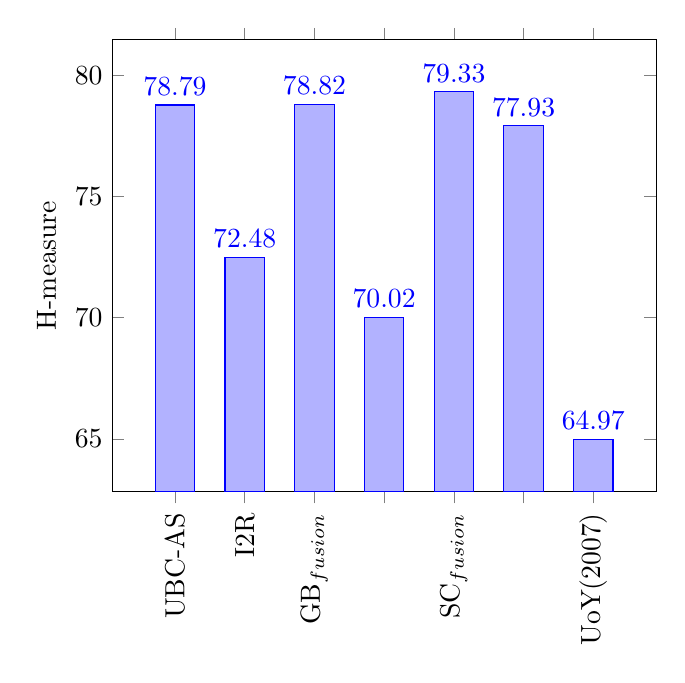
\begin{tikzpicture}{width=5cm,height=5cm}
\pgfplotsset{compat=1.8}
\begin{axis}[
%	xtick distance={160},
    ybar=-0.5cm,
    width=.7\linewidth,
    enlargelimits=0.15,
    domain = 0:30,
    xmin=0, xmax=30,
%    x=1mm, % Distance between the centers of the bars
%    enlarge x limits={abs=1cm}, % The distance between the center of the first bar and the left edge
%    enlarge y limits=false,
    legend style={at={(0.5,.97)},anchor=north,legend columns=-1},
    ylabel={H-measure},
%    xmin=0, xmax=85,
    xticklabels={
		UBC-AS,
		I2R,
		{GB$_{\text{fusion}}$},
		$\mlex$,
		{SC$_{\text{fusion}}$},
		$\msyn$,
		UoY(2007)
    },
    xtick={0,5,...,30},
    nodes near coords,
    nodes near coords align={vertical},
    x tick label style={rotate=90,anchor=east},
    ]
\addplot+[mark=none, bar width=.5cm]  coordinates {(0,78.79) (5,72.48) (10,78.82) (15,70.02) (20,79.33) (25,77.93) (30,64.97)};
%\legend{SF,1F,2F,HF}
\end{axis}
\end{tikzpicture}
\caption{H-measure for the WSI/WSD task on the Semeval 2007 corpus using our network-based method as well as other systems, indicated on the x-axis. The best performing system was spectral clustering with a fusion representation space SC$_{\text{fusion}}$.}
\label{fig:h_measure_semeval2007_nbased}
\end{figure}

We now look into the results from the H-measure perspective (see Figure \ref{fig:h_measure_semeval2007_nbased}). Again, as in the experiments with fusion opeartions, the best system SC$_{\text{fusion}}$ uses spectral clustering with a single cross media fusion operator, i.e., $X_F(\slex,\mlex)$. Close, in second place, we find the other fusion based system, this time using the network-based method proposed previously. Finally, the system UBC-AS  is ranked third by the H-measure.

In general, it is interesting to notice that the fusion operators outperform again the single features and is on pair with other performing systems. What does seems unexpected is that the roles played by the $\msyn$ and $\mlex$ system is inverted regarding to the fusion experiments presented in the previous subsection. Indeed, using our network-based approach the performance of $\msyn$ is considerably larger than that of $\mlex$, whereas using spectral clustering the lexical information outranked (by a small margin) the syntactic information (based on dependencies). Again, we attribute this lack of performance of $\mlex$ to the size of the window employed, which seems to general to detect appropriate senses.


As a way of determining where does both systems complement each other, in Figure \ref{fig:nouns_fs} and Figures  \ref{fig:verbs_fs2} and \ref{fig:verbs_fs3} we show the unsupervised F-measure value for nouns and verbs respectively (we split the verbs in two figures for visibility). We can see that, as the previous result tables indicated, $\msyn$ did better overall. Nonetheless, and what is most interesting in these figures, is that there are certain words (both nouns and verbs) that obtain better scores using $\mlex$ instead of $\msyn$ and vice versa. For example, the nouns \textit{area}, \textit{future}, and \textit{state} are better treated by $\mlex$, according to this measure, even if by a small margin. On the other hand, with respect to the verbs, the differences between performance are more important. Again, the $\mlex$ system does better while finding senses and assigning them to the verbs \textit{avoid}, \textit{fix}, and \textit{work}. %This information will be useful during the design of hybridization techniques between feature of our hypergraph structure.

 




 \begin{figure}[!htb]
\centering
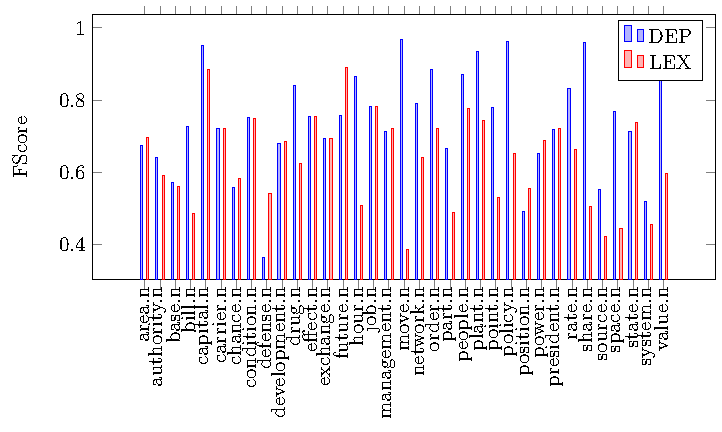
\includegraphics[width=1\linewidth]{images/Chapitre5/tex_img_files/nouns_fs.pdf}
\caption{Unsupervised F-measure results for the nouns of the Semeval 2007 test set.}
\label{fig:nouns_fs}
\end{figure}

 \begin{figure}[!htb]
\centering
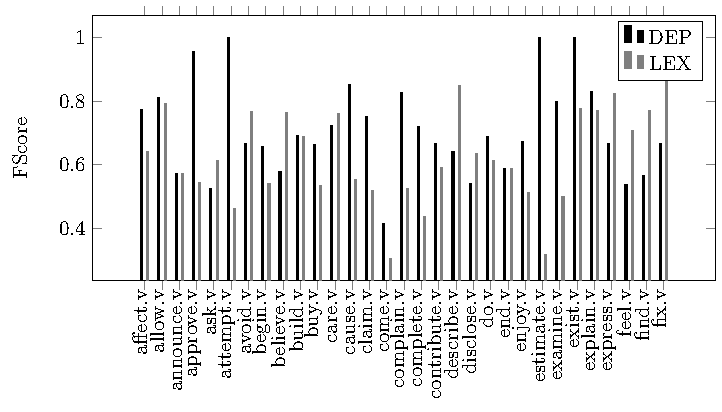
\includegraphics[width=1\linewidth]{images/Chapitre5/tex_img_files/verbs_fs_2.pdf}
\caption{Unsupervised F-measure results for the first half of verbs of the Semeval 2007 test set.}
\label{fig:verbs_fs2}
\end{figure}

 \begin{figure}[!htb]
\centering
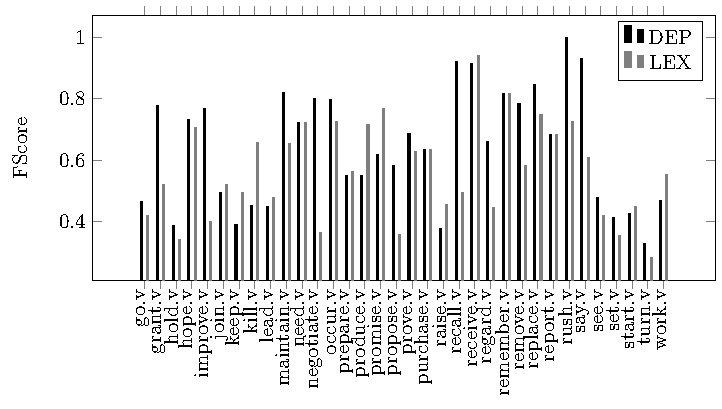
\includegraphics[width=1\linewidth]{images/Chapitre5/tex_img_files/verbs_fs_3.pdf}
\caption{Unsupervised F-measure results for the second half of verbs of the Semeval 2007 test set.}
\label{fig:verbs_fs3}
\end{figure}

%todo add phrase that says that syntactic is not as good as seen in the paper where they compare a lot of distributional models... 	


%todo split verbs?
\subparagraph{Semeval 2010}
In the Semeval 2010 dataset \cite{Semeval2010}, two unsupervised evaluation metrics are introduced: {V-measure} and {paired F-measure}. Briefly, the V-measure assesses the homogeneity or the quality of a clustering solution by measuring the degree to which each cluster consists of instances principally belonging to a single gold standard class. or homogeneity. It also takes into account completeness, or the level each gold standard class consists of instances primarily assigned to a single cluster. The V-measure is always greater than zero but it is not bounded to one as maximum value. We consider that the larger the measure, better. A well-known drawback is that the V-measure  is biased towards systems that yield many senses \cite{Semeval2010,VandeCruys2011,pedersen2010duluth}. We present this metric for completeness but we do not heavily base our conclusions on it.

On the other hand, the paired F-measure evaluation transforms the clustering problem into a classification. Two instance pairs sets are generated, the first one coming from the system induced clusters, by including pairs of the instances found in each cluster. The second set of instance pairs is built from the gold standard classes. It contains pairs of the instances found in each class. We can then define \textit{Precision} and \textit{Recall}. Precision is computed as the ratio of the number of common instance pairs between the two sets divided by the total number of pairs in the clustering solution. Recall is the count of common instance pairs between the two sets divided by the total number of pairs in the gold standard. The paired F-measure is the harmonic mean of both quantities.

Concerning the supervised evaluation, it follows the same of Semeval 2007, using recall as the main performance measure. The key difference is that the final results of the competition were obtained by reshuffling the data several times to avoid the issue of obtaining considerably different results with different splits of the data.

\begin{table}[]
\centering
\caption{Unsupervised V-measure  on the Semeval 2010 test set. The highest values for each column are in bold. Our results are obtained with our proposed algorithm.}
\begin{tabular}{@{}lrrrr@{}}
\toprule
\textbf{System} & \multicolumn{3}{c}{\textbf{V-measure (\%)}} & \textbf{\#cl} \\
 & \textbf{all} & \textbf{nouns} & \textbf{verbs} & \\ \midrule
{Hermit} & \textbf{16.2} & \textbf{16.7} & \textbf{15.6} & 10.8 \\
NMF$_{lib}$&11.8&13.5&9.4&4.8\\
$\mlex$ & 11.6 & 8.8 & 11.9 & 10.5 \\
Random & 4.4 & 4.2 & 4.6 & 4.0 \\
$\msyn$ & 3.5 & 3.9 & 2.8 & 2.8 \\
MFS & 0.0 & 0.0 & 0.0 & 1.0 \\ \bottomrule
\end{tabular}

\label{tab:sem2010_VM}
\end{table}

In Table \ref{tab:sem2010_VM} we present our systems compared to the baseline and other methods using during Semeval 2010. V-measure is a metric well-known for favoring systems producing a higher number of clusters \cite{VandeCruys2011,pedersen2010duluth}. Thus, it is considered not a very reliable metric. We have included it to have a global insight about the performance of our method. We remark that only $\mlex$ performed better than both baselines, random assignation of senses (Random) and using the most frequent sense (MFS). Also, we note that we included only the best performing systems, in this case NMF$_{lib}$ \cite{VandeCruys2011} and   Hermit \cite{JurgensS10}. The former  did not participate on the competition but was developed later. We include it henceforth to illustrate how systems variate from one position to another depending the metric used to assess the performance. The latter was the best method on this metric from the task challenge. It is important to notice that other systems exist between Hermit and $\mlex$. They were not included for the sake of clarity.

\begin{table}[]
\centering
\caption{Unsupervised Paired F-measure for the Semeval 2010 test set. The highest values for each column are in bold. Our results are obtained with our proposed algorithm.}
\begin{tabular}{@{}lrrrr@{}}
\toprule
\textbf{System} & \multicolumn{3}{c}{\textbf{Paired F-measure (\%)}} & \textbf{\#cl} \\
 & \textbf{all} & \textbf{nouns} & \textbf{verbs} & \\ \midrule

MFS & \textbf{63.5} & \textbf{57.0} & \textbf{72.4} & 1.0 \\
Duluth-WSI-SVD-Gap & 63.3 & \textbf{57.0} & \textbf{72.4} & 1.0 \\
$\msyn$ & 53.6 & 50.1 & 58.7 & 2.8 \\
NMF$_{lib}$&45.3&42.2&49.8&5.4\\
$\mlex$ & 38.4 & 46.7 & 28.5 & 10.5 \\
Random & 31.9 & 30.4 & 34.1 & 4.0 \\ \bottomrule
\end{tabular}

\label{tab:sem2010_FS}
\end{table}

The second unsupervised measure, Paired F-measure, can be seen in Table \ref{tab:sem2010_FS}. In this case both systems presented performed better than the random baseline. All the systems presented were able to beat the MFS baseline. We note that $\msyn$ does much better compared to $\mlex$ concerning verbs, namely 58\% vs. 28\% F-measure. Still, the results are low considering the best results of the competition, 63\% from the Duluth system \cite{Pedersen2010} , although again, it generates a number of senses very similar to the MFS baseline. Both our systems induce a considerable amount of clusters while keeping a descent F-measure. Our results are obtained with our proposed algorithm.



\begin{table}[!tb]
\centering
\caption{Supervised recall  for Semeval 2010 test set (80\% mapping, 20\% evaluation). The highest values for each column are in bold. Results are obtained with our proposed algorithm.}
\begin{tabular}{@{}lrrrr@{}}
\toprule
\textbf{System} & \multicolumn{3}{c}{\textbf{Recall (\%)}} & \textbf{\#cl}  \\
 & \textbf{all} & \textbf{nouns} & \textbf{verbs} & \\ \midrule
%\textbf{Recall (\%)} & \textbf{all} & \textbf{nouns} & \textbf{verbs} \\ \midrule
NMF$_{lib}$&\textbf{62.6}&57.3&\textbf{70.2} & 5.4\\
UoY(2010) & 62.4 & \textbf{59.4} & 66.8 & 11.5\\

$\mlex$ & 59.8 & 55.8 & 67.4 & 10.5\\
$\msyn$ & 59.3 & 53.9 & 67.2 & 2.8\\
MFS & 58.7 & 53.2 & 66.6 & 1.0\\
Random & 57.3 & 51.5 & 65.7 & 4.0\\ \bottomrule

\end{tabular}


\label{tab:sem2010_SR}
\end{table}


Finally, we in Table \ref{tab:sem2010_SR} we show the supervised Recall results of Semeval 2010. The best performing algorithm shown is NMF$_{lib}$. During the competition, UoY(2010) was the best method. It is a graph-based algorithm which shares the name with the UoY(2007)  system presented in Semeval 2007, but it is a different  approach. Concerning our systems, in this evaluation they seem to perform the best, or in a comparable level, to the top methods.  We find that in general our systems seem to perform better on the Semeval 2007 dataset. Discovering the reason could shed light into improving the performance on the Semeval 2010 test set. Given the results, it seems like a combination of features (syntactic plus lexical) in  a single algorithm could yield better results. 

Again, in order to find the overall best systems, we present the H-measure as before. This time the H-measure will be the harmonic mean of the newly introduced unsupervised paired F-measure instead of the plain F-measure used before. The supervised recall stays also as before. We do not employ the V-measure for the reasons exposed before, namely it is biased towards systems that generate many senses. Ideally, the paired F-measure was conceived to punish systems that produced less or more senses than the true average number of senses for each target word. In reality, it does not seem to be the case. We present in Figure \ref{fig:h_measure_semeval2010} the H-measure ($\delta=3.79$) results for the systems discussed previously in the Semeval 2010 context. Duluth-WSI-SVD-Gap is the best system overall, followed by our approach using $\msyn$ as input matrix. 

Looking at the results, we argue that the Semeval 2010 task was more complex than Semeval 2007. We believe it is in part due to the fact that there are more verbs in the dataset, which are always harder to disambiguate than nouns. The dataset was also considerably larger, which may have introduced noise and required more sophisticated filtering techniques. We see that our system $\mlex$ performs poorly. Indeed, it generates too many senses, which is a symptom of poorly generated clusters, that is, the clusters found are not distinctive nor cohesive enough to enclose whole senses. On the other hand $\msyn$ does reasonably well, maybe in part due to the fact that again there are more verbs whose senses are better distinguished   using syntactic information.



\begin{figure}
\centering
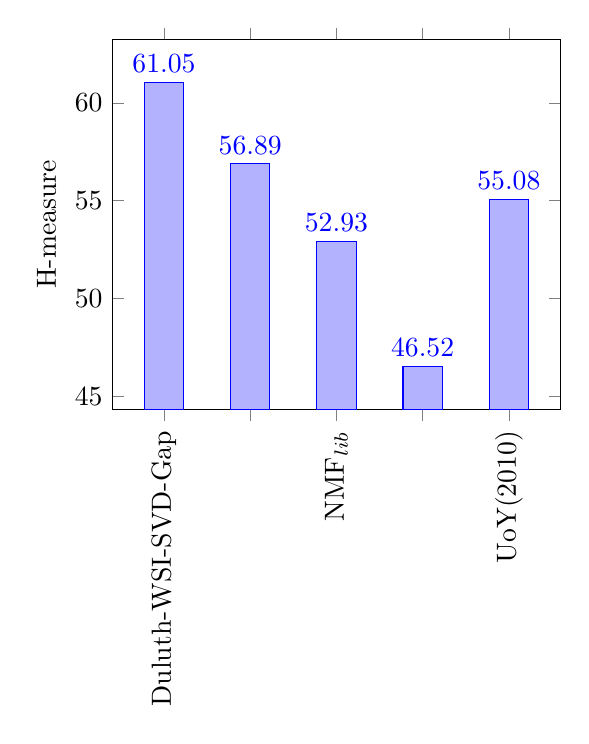
\begin{tikzpicture}{width=5cm,height=5cm}
\pgfplotsset{compat=1.8}
\begin{axis}[
%	xtick distance={160},
    ybar=-0.5cm,
    width=.6\linewidth,
    enlargelimits=0.15,
    domain = 0:20,
    xmin=0, xmax=20,
%    x=1mm, % Distance between the centers of the bars
%    enlarge x limits={abs=1cm}, % The distance between the center of the first bar and the left edge
%    enlarge y limits=false,
    legend style={at={(0.5,.97)},anchor=north,legend columns=-1},
    ylabel={H-measure},
%    xmin=0, xmax=85,
    xticklabels={
		Duluth-WSI-SVD-Gap,
		$\msyn$,
		{NMF$_{\text{lib}}$},
		$\mlex$,
		UoY(2010)
    },
    xtick={0,5,...,20},
    nodes near coords,
    nodes near coords align={vertical},
    x tick label style={rotate=90,anchor=east},
    ]
\addplot+[mark=none, bar width=.5cm]  coordinates {(0,61.05) (5,56.89) (10,52.93) (15,46.52) (20,55.08)};
%\legend{SF,1F,2F,HF}
\end{axis}
\end{tikzpicture}
\caption{H-measure for the WSI/WSD task on the Semeval 2010 corpus using our network-based method as well as other systems, indicated on the x-axis. The best performing system is Duluth-WSI-SVD-Gap, while our best method is that based on syntactic information $\msyn$.}
\label{fig:h_measure_semeval2010}
\end{figure}





%\paragraph{Conclusion}

\section{Conclusion}
\label{chap6:conclusion}
In this chapter we addressed two NLP tasks from two different points of view: on the one hand, we computed several representation spaces using fusion operations in order to enrich and densify otherwise sparse and independent features. The matrices generated were used to train both supervised and unsupervised models to solve named entity recognition and word sense induction and disambiguation.

On the other hand, we proposed a model that leverages the inner structure of the hypergraph network to group words that belong to a shared sense. This approach was used to solve word sense induction.

More specifically, concerning the first part, we presented  a comparative study of multimedia fusion techniques applied to named entity recognition.  We also tested hybrid fusion recombinations in order to complement the information contained in the single representation matrices. In order to accomplish this goal, we built upon basic fusion techniques such as early and late fusion, as well as cross media fusion to transfer quality information from one set of features to another. 

%We found that by taking a strong feature, in our case lexical context, $\mlex$, and enriching it with the output of rather complex fusion combinations, we can improve the performance of the tasks addressed. The enrichment has to give more relevance to the strong feature matrix, by selecting the right parameters. 

We analyzed the results to understand how the enrichment of features improved the performance. We found that at each fusion step, a different type of NER tag is benefited. We studied what features where driving the decision towards the correct class and found that while the enriched features are not the most prominent  in the decision function, they play an important role by tipping said decision towards the correct label and away from the wrong one. 

Concerning fusion enrichment and WSI/WSD, we found that the fusion operations also improve the results of the task, although not as clearly as in NER. The metrics used to measure the performance on this ask does not allow a clear understanding on the behavior of the model employed. While we want to avoid converging to the trivial one sense per word solution, we know that words do not have numerous senses. In that sense, the results obtained stay reasonably away from the trivial solution while not producing many senses as other approaches.

We proposed a metric, the H-measure, to rank the systems by considering the classic performance metrics and the number of senses found relative to the true number of senses. This metric allowed us to identify with a single value the best system. We found that according to it, the fusion based systems, whether using well-known algorithms (spectral clustering) or using the method developed in this section, perform adequately and show general improvements over the single feature representations as well as other systems.

While there is an improvement using fusion techniques, we do note that they  enlarge the feature space, especially early fusion, which is used frequently. This may imply the need of larger quantities of memory and longer execution time. In that sense, as future work, more intelligent ways of finding the most appropriate fusion must be researched. This is indeed one of our future work paths: determining an optimal fusion path from single features to a high degree fusion recombination. Coupled with this, the automatic determination of the parameters is still ongoing research in the multimedia fusion community. Consequently, we believe that efficiently determining both parameters and fusion combinations is the general domain of our future work. Another route we would like to explore is testing these techniques on other tasks and with datasets from different domains, in order to assert its effectiveness.


% WSD network
Concerning our proposed network-based method, we show how using the inner links within the hypergraph structure we can group words that represent senses and then assign them to target words. Our method distinguishes from similar works in two main aspects: the definition of similarity used, the reduced number of parameters that are needed, the use of diverse types of contexts to solve the task. 	We show that our method beats said similar approaches. Also, we discovered the behavior of syntactic contexts in comparison to lexical contexts at word-level. Indeed, lexical contexts seem to perform better. This is in line with other works on distributional representations \cite{kiela2014systematic}.



%\minitoc

%\subsubsection{Introduction}
